% ============================================================
% Chapter 6 --- Compactness
% Originally: content/week-02.tex, \section{Compactness} (Corsin Week 2, Friday)
%           + content/week-03.tex, \section{Compactness --- continued} and
%             \subsection{Why do we care about compactness?} (Corsin Week 3, Monday)
%
% These were one topic split across two teaching weeks, joined in the old files by a
% \section{Compactness --- continued} heading and a \continuedfrom back-pointer. Both are
% gone: the material is continuous here, so nothing needs to point backwards.
% ============================================================
\chapter{Compactness}
\label{ch:compactness}

% Transition: Claude Opus 5 (Medium)
Compactness is the least self-explanatory definition in this part, so it is worth saying in
advance what it is \emph{for}. Finite sets are easy to handle: one can take a maximum, choose a
smallest radius, check finitely many cases. Infinite sets are not. Compactness is the property
that lets an infinite space be treated as if it were finite --- not because it is small, but
because every attempt to spread it out over infinitely many open pieces collapses back to
finitely many.

The chapter defines compactness by open covers, proves it equivalent to sequential compactness,
records the Heine--Borel theorem for $\mathbb{R}^n$ and how badly it fails elsewhere, and closes
with the three payoffs that make the definition worth having.

% Originally: content/week-02.tex, \section{Compactness} (Corsin Week 2, Friday)

\section{Compactness}
\label{sec:compactness}

% Transition: Claude Opus 5 (High)
Compactness is the least self-explanatory definition in this chapter, so it is worth saying in
advance what it is \emph{for}. Finite sets are easy to handle: one can take a maximum, choose a
smallest radius, check finitely many cases. Infinite sets are not. Compactness is the property
that lets an infinite space be treated as if it were finite --- not because it is small, but
because every attempt to spread it out over infinitely many open pieces collapses back to
finitely many. \Cref{sec:why_compactness_matters} collects the three payoffs
(continuous images, attained extrema, uniform continuity); the definition below is what buys
them.

\begin{definition}[Compact metric space]
\label{def:compact_metric_space}
A metric space $(X,d)$ is \newterm{compact} (\germanterm{kompakt}) if every open cover
(by sets open in the sense of \cref{def:open_closed}) has a finite subcover.
\end{definition}

\begin{notation}[Open covers]
\label{not:open_cover}
An \newterm{open cover} (\germanterm{offene \"Uberdeckung}) of $X$ is a family
$\{U_i\}_{i \in I}$ of open sets with $X = \bigcup_{i\in I}U_i$; the index set $I$ is allowed to
be arbitrary, in particular uncountable. A \newterm{subcover} is a subfamily
$\{U_i\}_{i \in J}$, $J \subseteq I$, that still covers $X$, and it is \emph{finite} when $J$
is. The order of quantifiers is what carries the content: \emph{every} cover must admit
\emph{some} finite subcover. Exhibiting one cover with a finite subcover proves nothing --- any
space has the cover $\{X\}$ --- whereas exhibiting one cover \emph{without} a finite subcover
disproves compactness outright, which is how \cref{ex:heine_borel_fails} and the
open-interval example below both work.
\end{notation}

% Source: Corsin Nick/Class Notes/Week 2.pdf, pp. 1--13

\begin{theorem}[Sequential compactness]
\label{thm:sequential_compactness}
A metric space $(X,d)$ is compact if and only if every sequence in $X$ has a convergent
(\cref{def:convergent_sequence}) subsequence in $X$.
\end{theorem}

\begin{ainote}
Neither Corsin nor the official lecture notes prove this here; the proof is given below as
\Cref{thm:sequential_topological_compactness_equivalence}, once the tools it needs (total
boundedness) are available.
\end{ainote}

\begin{center}
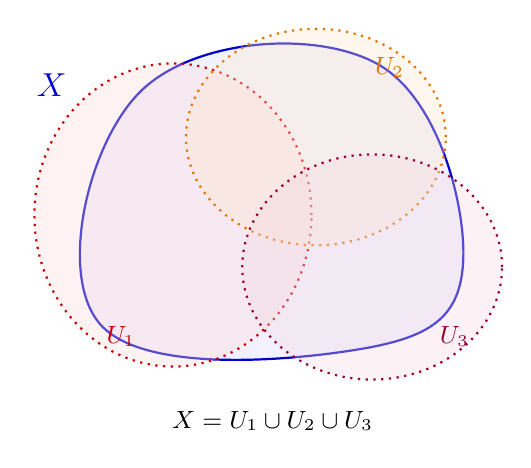
\begin{tikzpicture}[scale=1.1]
  \draw[blue!80!black, thick, fill=blue!5] plot[smooth cycle, tension=0.7] coordinates {(-2, -1.2) (-1.5, 1.5) (1.2, 1.8) (2.2, -0.5) (1.0, -1.5)};
  \node[blue!80!black, font=\large] at (-2.55, 1.55) {$X$};

  % The three sets must genuinely cover X -- ellipses chosen so every point of the
  % blob lies inside at least one of them (that is the whole point of a cover).
  \draw[red!80!black, thick, dotted, fill=red!15, fill opacity=0.35] (-1.15,0.05) ellipse (1.6 and 1.75);
  \node[red!80!black, font=\small] at (-1.75, -1.35) {$U_1$};

  \draw[orange!90!black, thick, dotted, fill=orange!20, fill opacity=0.35] (0.5,0.95) ellipse (1.5 and 1.25);
  \node[orange!90!black, font=\small] at (1.35, 1.75) {$U_2$};

  \draw[purple!80!black, thick, dotted, fill=purple!15, fill opacity=0.35] (1.15,-0.55) ellipse (1.5 and 1.3);
  \node[purple!80!black, font=\small] at (2.1, -1.35) {$U_3$};

  \node[below, font=\small] at (0, -2.1) {$X = U_1 \cup U_2 \cup U_3$};
\end{tikzpicture}
\end{center}

% Sonnet 5 (Medium)

% Originally: content/week-02.tex, \subsection{Compact subsets} (Corsin Week 2, Friday)

\subsection{Compact subsets}

A subset $K$ of a metric space $(X,d)$ is compact if the metric space $(K, d|_{K \times K})$ is
compact (\cref{def:compact_metric_space}). This is equivalent to the definition in the script:

\begin{definition}[9.63, quoted from the official lecture notes]
\label{def:sequential_topological_compactness}
Let $(X,d)$ be a metric space. A subset $K \subset X$ is called \textbf{compact} if one of the
following equivalent conditions hold:
\begin{enumerate}[label=\textbf{(\alph*)}]
  \item \label{item:seq_compact_def963}
    $K$ is \textbf{sequentially compact}: every sequence $(x_n)_{n\in\mathbb{N}}$ in $K$ has
    a subsequence that is convergent (\cref{def:convergent_sequence}) in $K$.
  \item \label{item:top_compact_def963}
    $K$ is \textbf{topologically compact}: every family of open sets
    (\cref{def:open_closed}) $\{U_i\}_{i \in I}$ that cover $K$, has a finite subcover.
\end{enumerate}
\end{definition}

\begin{center}
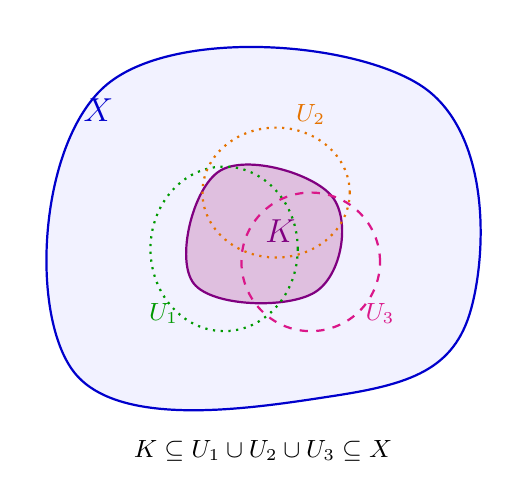
\begin{tikzpicture}[scale=1.1]
  \draw[blue!80!black, thick, fill=blue!5] plot[smooth cycle, tension=0.7] coordinates {(-2.2, -1.5) (-1.8, 1.8) (1.8, 1.8) (2.4, -0.8) (0.8, -1.8)};
  \node[blue!80!black, font=\large] at (-1.9, 1.5) {$X$};

  \draw[violet, thick, fill=violet!25] plot[smooth cycle, tension=0.7] coordinates {(-0.8, -0.5) (-0.5, 0.8) (0.8, 0.5) (0.6, -0.6)};
  \node[violet, font=\large] at (0.2, 0.1) {$K$};

  % As above: the three sets must cover all of K (they need not, and here do not,
  % cover all of X -- that is exactly the difference between the two pictures).
  \draw[green!60!black, thick, dotted] (-0.45,-0.1) ellipse (0.85 and 0.95);
  \node[green!60!black, font=\small] at (-1.15, -0.85) {$U_1$};

  \draw[orange!90!black, thick, dotted] (0.15,0.55) ellipse (0.85 and 0.75);
  \node[orange!90!black, font=\small] at (0.55, 1.45) {$U_2$};

  \draw[magenta!90!black, thick, dashed] (0.55,-0.25) ellipse (0.8 and 0.8);
  \node[magenta!90!black, font=\small] at (1.35, -0.85) {$U_3$};

  \node[below, font=\small] at (0, -2.2) {$K \subseteq U_1 \cup U_2 \cup U_3 \subseteq X$};
\end{tikzpicture}
\end{center}

% Quelle: Diego Torres Tejeda/Addendum - Sequential and Topological Compactness.pdf -- Sonnet 5 (Medium)

% Originally: content/week-02.tex, \subsection{Sequential and topological compactness agree}

\subsection{Sequential and topological compactness agree}

% Diego Torres Tejeda's supplementary note "Addendum - Sequential and Topological Compactness.pdf"
% is the one typeset document among his materials, the rest being handwritten scans. Its proof is
% adapted below into this project's notation and house style.
\begin{ainote}
Neither this equivalence nor \cref{thm:sequential_compactness} above is proved in the
transcribed notes. A complete, self-contained proof is supplied here
from a second tutor's addendum. By the reduction already noted above, compactness of
$K \subseteq X$ being compactness of the metric space $(K,d|_{K\times K})$, it suffices to treat a
whole metric space $X$ rather than a subset $K$.
\end{ainote}

\begin{lemma}[Continuous functions attain extrema on sequentially compact spaces]
\label{lem:sequential_compactness_extreme_values}
Let $(X,d)$ be sequentially compact (\cref{item:seq_compact_def963}) and $f : X \to \mathbb{R}$
continuous. Then $f$ attains a maximum and a minimum on $X$.
\end{lemma}

\begin{proof}
It suffices to find a minimum (apply the result to $-f$ for the maximum). Let
$m := \inf_{x\in X} f(x) \in [-\infty,\infty)$ and choose a sequence $(x_n)_{n}$ with
$f(x_n) \to m$. By sequential compactness, some subsequence $x_{n_k} \to x \in X$; by continuity,
$f(x) = \lim_k f(x_{n_k}) = m$. In particular $m \neq -\infty$, so $f$ attains its minimum $m$ at
$x$.
\end{proof}

\begin{remark}
This is exactly the extreme value theorem (\cref{item:extreme_value_theorem}) proved from first
principles, without presupposing \cref{thm:sequential_compactness}. Avoiding that appeal is
essential here, since that theorem is precisely what we are about to prove.
\end{remark}

\begin{definition}[Totally bounded]
\label{def:totally_bounded}
A metric space $(X,d)$ is \newterm{totally bounded} \germanfor{total beschr\"ankt} if for
every $\varepsilon > 0$ there exist finitely many points $x_1,\dots,x_n \in X$ such that
\[X = \bigcup_{k=1}^{n} B_\varepsilon(x_k).\]
\end{definition}

% Supplement: Analysis_II_Script_v1.pdf, p. 22
\begin{exercise}[Totally bounded is strictly stronger than bounded]
\label{ex:totally_bounded_implies_bounded}
Let $X$ be a metric space. Show that if $X$ is totally bounded, then it is bounded, i.e.\
$\sup_{x,x'\in X}d(x,x') < \infty$. Find an example of a bounded metric space that is
\emph{not} totally bounded.
\end{exercise}

\begin{exercisesolution}[Proof of \cref{ex:totally_bounded_implies_bounded}]
% Generator: Claude Sonnet 5 (High)
\textbf{Totally bounded $\Rightarrow$ bounded.} Apply \cref{def:totally_bounded} with
$\varepsilon := 1$: there are $x_1,\dots,x_n$ with $X = \bigcup_{k=1}^n B_1(x_k)$. Let
$M := \max_{i,j}d(x_i,x_j)$ (finite, a maximum over finitely many pairs). For any
$x,x' \in X$, choose $i,j$ with $x \in B_1(x_i)$, $x' \in B_1(x_j)$; the triangle inequality
gives $d(x,x') \leq d(x,x_i)+d(x_i,x_j)+d(x_j,x') < 1+M+1$, so $X$ is bounded.

\textbf{Not conversely.} Let $X$ be any infinite set with the discrete metric. Then
$\sup_{x,x'}d(x,x') = 1 < \infty$, so $X$ is bounded. But $X$ is not totally bounded: for
$\varepsilon := \tfrac12$, every ball $B_{1/2}(x) = \{x\}$ (\cref{def:open_ball}), so no
\emph{finite} union of such balls can cover the infinite set $X$.
\end{exercisesolution}

\begin{remark}
This is the same asymmetry \cref{lem:sequentially_compact_totally_bounded} proves in one
direction only: sequential compactness forces \emph{both} boundedness and total boundedness, and
this exercise shows the two are genuinely different hypotheses. Total boundedness is the strictly
stronger of the two, and the gap opens up in infinite dimensions.
\end{remark}

\begin{lemma}[Sequential compactness gives (total) boundedness]
\label{lem:sequentially_compact_totally_bounded}
Let $(X,d)$ be sequentially compact. Then $X$ is bounded and totally bounded
(\cref{def:totally_bounded}).
\end{lemma}

\begin{proof}
\textbf{Bounded.} Fix $x_0 \in X$; the function $f(y) := d(x_0,y)$ is continuous, so by
\Cref{lem:sequential_compactness_extreme_values} it attains a maximum $M \geq 0$ on $X$. Then
$X = B_{M+1}(x_0)$.

\textbf{Totally bounded.} Fix $\varepsilon > 0$. Construct a sequence inductively: let
$x_1 \in X$ be arbitrary, and, having chosen $x_1,\dots,x_n$, let
$U_n := \bigcup_{k=1}^n B_\varepsilon(x_k)$. If $U_n = X$, stop, since we then have the desired
finite cover. Otherwise pick $x_{n+1} \in X\setminus U_n$, so that $d(x_{n+1},x_k) \geq \varepsilon$ for
all $k \leq n$. If this process never terminates, sequential compactness gives a convergent, hence
Cauchy, subsequence $(x_{n_k})_k$; but $d(x_{n_k},x_{n_{k+1}}) \geq \varepsilon$ for all $k$
contradicts the Cauchy property. So, the process must terminate after finitely many steps, giving
the desired finite $\varepsilon$-net.

% Sonnet 5 (Medium)
\begin{center}
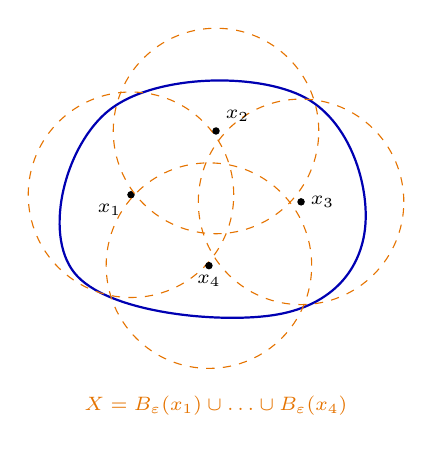
\begin{tikzpicture}[scale=0.9]
  \draw[blue!70!black, thick] plot[smooth cycle, tension=0.7] coordinates
    {(-2,-1) (-1.5,1.3) (1.2,1.5) (2.1,-0.4) (0.8,-1.6)};
  % Total boundedness means the finitely many balls really do cover X, so the
  % radius must be large enough to reach the corners of the blob.
  \foreach \p in {(-1.2,0.1),(0.0,1.0),(1.2,0.0),(-0.1,-0.9)} {
    \fill \p circle (1.5pt);
    \draw[orange!90!black, dashed] \p circle (1.45);
  }
  \node[font=\scriptsize, below left] at (-1.2,0.1) {$x_1$};
  \node[font=\scriptsize, above right] at (0.0,1.0) {$x_2$};
  \node[font=\scriptsize, right] at (1.2,0.0) {$x_3$};
  \node[font=\scriptsize, below] at (-0.1,-0.9) {$x_4$};
  \node[font=\scriptsize, orange!90!black, below] at (0,-2.6) {$X = B_\varepsilon(x_1)\cup\dots\cup B_\varepsilon(x_4)$};
\end{tikzpicture}
\end{center}
\end{proof}

\begin{theorem}[Sequential and topological compactness agree]
\label{thm:sequential_topological_compactness_equivalence}
A metric space $(X,d)$ is sequentially compact (\cref{item:seq_compact_def963}) if and only if it
is topologically compact (\cref{def:compact_metric_space}). In particular,
\Cref{thm:sequential_compactness} holds.
\end{theorem}

\begin{proof}
\textbf{($\Leftarrow$)} Suppose $X$ is not sequentially compact, so some sequence
$(x_n)_{n\in\mathbb{N}}$ has no convergent subsequence. Then no $x \in X$ is the limit of any
subsequence, so there exist $\varepsilon_x > 0$ and $N_x \in \mathbb{N}$ such that
$B_{\varepsilon_x}(x) \cap \{x_n : n \geq N_x\} = \emptyset$. The balls
$\{B_{\varepsilon_x}(x)\}_{x \in X}$ cover $X$, so topological compactness gives finitely many
$x_1,\dots,x_m$ with $X = \bigcup_{k=1}^m B_{\varepsilon_{x_k}}(x_k)$. With
$N := \max\{N_{x_1},\dots,N_{x_m}\}$, every $x_n$ with $n \geq N$ then avoids
$B_{\varepsilon_{x_1}}(x_1) \cup \dots \cup B_{\varepsilon_{x_m}}(x_m) = X$, which is absurd.
Therefore, $X$ is sequentially compact.

\begin{center}
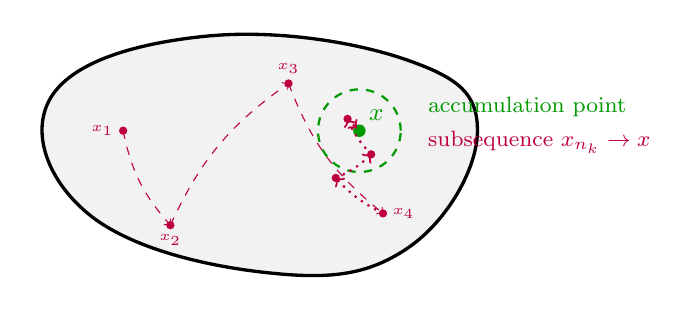
\begin{tikzpicture}[scale=1.5]
  % Space K
  \draw[very thick, fill=gray!10] plot[smooth cycle, tension=0.7] coordinates {(-1.5, -0.5) (-1.8, 0.5) (-0.5, 1) (1.2, 0.8) (1.8, 0.2) (1.2, -0.8) (0, -1)};
  
  % Sequence points and path
  \fill[purple] (-1.2, 0.2) circle (1pt) node[left] {\tiny $x_1$};
  \fill[purple] (-0.8, -0.6) circle (1pt) node[below] {\tiny $x_2$};
  \fill[purple] (0.2, 0.6) circle (1pt) node[above] {\tiny $x_3$};
  \fill[purple] (1.0, -0.5) circle (1pt) node[right] {\tiny $x_4$};
  \draw[->, purple, dashed] (-1.2, 0.2) to[bend right=15] (-0.8, -0.6);
  \draw[->, purple, dashed] (-0.8, -0.6) to[bend left=15] (0.2, 0.6);
  \draw[->, purple, dashed] (0.2, 0.6) to[bend right=15] (1.0, -0.5);
  
  % Accumulation point
  \fill[green!60!black] (0.8, 0.2) circle (1.5pt) node[above right] {\small $x$};
  \draw[green!60!black, dashed, thick] (0.8, 0.2) circle (0.35);
  
  % Subsequence converging
  \fill[purple] (0.6, -0.2) circle (1pt);
  \fill[purple] (0.9, 0) circle (1pt);
  \fill[purple] (0.7, 0.3) circle (1pt);
  \draw[->, purple, dotted, thick] (1.0, -0.5) to[bend left=10] (0.6, -0.2);
  \draw[->, purple, dotted, thick] (0.6, -0.2) to[bend right=10] (0.9, 0);
  \draw[->, purple, dotted, thick] (0.9, 0) to[bend left=10] (0.7, 0.3);
  \draw[->, purple, dotted, thick] (0.7, 0.3) -- (0.78, 0.22);
  
  \node[green!60!black, anchor=west] at (1.3, 0.4) {\footnotesize accumulation point};
  \node[purple, anchor=west] at (1.3, 0.1) {\footnotesize subsequence $x_{n_k} \to x$};
\end{tikzpicture}
\end{center}

\textbf{($\Rightarrow$)} Suppose $X$ is sequentially compact and let $\{U_i\}_{i\in I}$ be an open
cover; we may assume no single $U_i$ equals $X$ (else $\{U_i\}$ is itself a finite subcover).
Define
\[r(x) := \tfrac12\sup\{r \geq 0 : B_r(x) \subseteq U_i \text{ for some } i \in I\}, \qquad x \in X.\]
\textit{$r$ is finite and positive.} Since $\{U_i\}$ covers $X$ and each $U_i$ is open, some
$U_{i_0} \ni x$ contains a ball around $x$, so $r(x) > 0$; and since $X$ is bounded
(\cref{lem:sequentially_compact_totally_bounded}) but no $U_i$ equals $X$, $r(x) < \infty$.

\textit{$r$ is Lipschitz, hence continuous.} (That is, $|r(x)-r(y)| \leq L\,d(x,y)$ for a
constant $L$; the notion is named and placed in context as \cref{def:lipschitz_continuous},
but only the displayed estimate is used here.) Write
$R(x) := \sup\{\rho \geq 0 : B_\rho(x) \subseteq U_i \text{ for some } i\}$, so that
$r = \tfrac12 R$; it is $R$ that the argument bounds, and the factor $\tfrac12$ must be carried
through.

Let $x,y \in X$ with $d(x,y) < r(x)$. Since $r(x) < R(x)$, we have
$B_{r(x)}(x) \subseteq U_i$ for some $i$, so $y \in U_i$, and the triangle inequality gives
\[B_{r(x)-d(x,y)}(y) \subseteq B_{r(x)}(x) \subseteq U_i
\qquad\Longrightarrow\qquad R(y) \geq r(x)-d(x,y).\]
Halving, $r(y) = \tfrac12R(y) \geq \tfrac12\big(r(x)-d(x,y)\big)$, which also holds trivially
when $d(x,y) \geq r(x)$ since $r(y) \geq 0$. By symmetry,
\[|r(x)-r(y)| \leq \tfrac12\,d(x,y),\]
so $r$ is $\tfrac12$-Lipschitz, and in particular continuous, which is all that is needed below.

By \cref{lem:sequential_compactness_extreme_values}, $r$ attains a minimum
$\varepsilon := \min_{x\in X} r(x) > 0$ on $X$. Then $B_\varepsilon(x) \subseteq U_i$ for some $i$,
for every $x \in X$. By \cref{lem:sequentially_compact_totally_bounded}, $X$ is totally bounded,
so there are $x_1,\dots,x_n \in X$ with $X = \bigcup_{k=1}^n B_\varepsilon(x_k)$; choosing, for
each $k$, an index $i_k$ with $B_\varepsilon(x_k) \subseteq U_{i_k}$, the sets
$U_{i_1},\dots,U_{i_n}$ form a finite subcover of $X$.
\end{proof}

\begin{remark}[Total boundedness, more generally]
\label{rem:compact_iff_complete_totally_bounded}
Diego's note records a sharper characterization as a further exercise: $(X,d)$ is compact if and
only if it is complete and totally bounded. \Cref{lem:sequentially_compact_totally_bounded} gives
one direction (compact $\implies$ complete, by \cref{ex:compact_finite_complete} below, and
totally bounded); for the converse, a Cauchy subsequence can be extracted from any sequence using
total boundedness (cover by finitely many $\tfrac1k$-balls for $k=1,2,\dots$ and pass to nested
subsequences), and it converges by completeness.
\end{remark}

% Quelle: Diego Torres Tejeda/Addendum - Sequential and Topological Compactness.pdf, \S4(b)
\begin{definition}[Lebesgue number]
\label{def:lebesgue_number}
Let $(X,d)$ be a metric space and $\{U_i\}_{i\in I}$ an open cover of $X$. A number
$\varepsilon > 0$ is a \newterm{Lebesgue number} \germanfor{Lebesgue-Zahl} for the cover if
\[\forall x \in X\ \exists i \in I: B_\varepsilon(x) \subseteq U_i.\]
\end{definition}

\begin{remark}[Lebesgue's covering lemma]
The proof of \cref{thm:sequential_topological_compactness_equivalence} ($\Rightarrow$) shows
more than stated: on a compact metric space, \emph{every} open cover has a Lebesgue number (take
$\varepsilon := \min_{x\in X} r(x)$ as constructed there). This is known as \newterm{Lebesgue's
covering lemma} \germanfor{Lebesguesches \"Uberdeckungslemma}.
\end{remark}

\begin{proposition}[Compactness implies uniform continuity]
\label{prop:compact_implies_uniformly_continuous}
Let $(X,d_X)$, $(Y,d_Y)$ be metric spaces with $X$ compact, and let $f : X \to Y$ be continuous.
Then $f$ is uniformly continuous (\cref{def:uniformly_continuous}).
\end{proposition}

\begin{proof}
% Generator: Claude Sonnet 5 (Medium), after Diego Torres Tejeda/Addendum, §4(b)
Let $\varepsilon > 0$. The sets $f^{-1}(B_{\varepsilon/2}(y))$, $y \in Y$, are open
(\cref{def:continuous}) and cover $X$, so they admit a Lebesgue number $\delta > 0$
(\cref{def:lebesgue_number}). For any $x,x' \in X$ with $d_X(x,x') < \delta$, the ball
$B_\delta(x)$ lies inside some $f^{-1}(B_{\varepsilon/2}(y))$, so $x' \in B_\delta(x)$ gives
$f(x),f(x') \in B_{\varepsilon/2}(y)$, hence $d_Y(f(x),f(x')) < \varepsilon$ by the triangle
inequality. Since $\delta$ did not depend on $x$, $f$ is uniformly continuous.
\end{proof}

% Supplement: Sascha Brack/Class Notes/Week_02_Notes_Friday_Updated.pdf, p. 6
\begin{proposition}[A closed subset of a compact set is compact]
\label{prop:closed_subset_of_compact}
Let $(X,d)$ be a metric space, $K \subseteq X$ compact, and $A \subseteq K$ closed in $X$. Then
$A$ is compact.
\end{proposition}

\begin{proof}
Let $\mathcal{U}$ be an open cover of $A$. Since $A$ is closed, $X\setminus A$ is open, so
\[\mathcal{U}' := \mathcal{U} \cup \{X\setminus A\}\]
is an open cover of $K$, covering $A$ by assumption and everything outside $A$ by the added
set. Compactness of $K$ gives a finite subcover
$U_{1},\dots,U_{m} \in \mathcal{U}'$ of $K$, hence of $A$.

\begin{center}
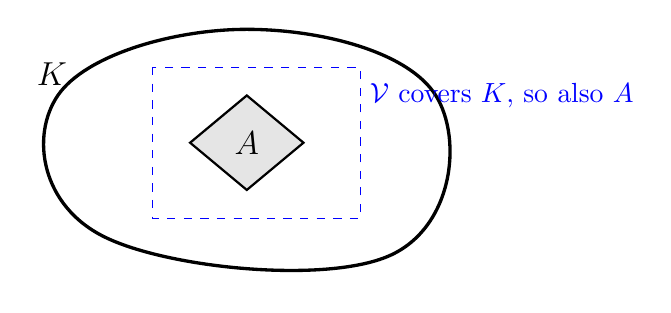
\begin{tikzpicture}[scale=1.2]
  % Compact set K
  \draw[very thick] plot[smooth cycle, tension=0.7] coordinates {(-1.5, -1) (-2, 0.5) (0, 1.2) (2, 0.5) (1.5, -1.2)};
  \node[above left, font=\large] at (-1.8, 0.5) {$K$};
  
  % Closed set A
  \draw[thick, fill=gray!20] (0, 0.5) -- (-0.6, 0) -- (0, -0.5) -- (0.6, 0) -- cycle;
  \node[font=\large] at (0, 0) {$A$};
  
  % Open cover V
  \draw[dashed, blue] (-1, 0.8) rectangle (1.2, -0.8);
  \node[blue, right] at (1.2, 0.5) {$\mathcal{V}$ covers $K$, so also $A$};
\end{tikzpicture}
\end{center}

Now simply discard $X\setminus A$ from that list if it occurs: it contains no point of $A$, so
the remaining sets still cover $A$. They all belong to $\mathcal{U}$, and there are finitely
many. As $\mathcal{U}$ was arbitrary, $A$ is compact.
\end{proof}

% Reclassified from ainote to remark: a proof technique worth naming is mathematics.
\begin{remark}[Enlarge the cover, then discard the extra set]
The trick just used is the standard way to transfer compactness downward, and it is worth
remembering in the form \emph{enlarge the cover by the complement of the set you care about, then
throw that complement away again}. It reappears whenever one needs a compact subset of a compact
set. Note that the hypothesis \qt{closed} is essential, since $(0,1) \subseteq [0,1]$ sits inside
a compact set without being compact.
\end{remark}

% Source: Corsin Nick/Class Notes/Week 2.pdf, p. 15
\begin{exercise}[Compact sets are complete]
\label{ex:compact_finite_complete}
Let $(X,d)$ be a metric space.
\begin{enumerate}[label=\textbf{(\alph*)}]
  \item Show that every finite subset $\{x_1, \dots, x_n\} \subseteq X$ is compact.
  \item If $X$ is compact, is it complete (\cref{def:complete_metric_space})?
\end{enumerate}
\end{exercise}

% Kept inline: solved directly in Corsin Nick/Class Notes/Week 2.pdf, p. 15. (The chapter-level
% "pp. 1--13" Source comment above predates this exercise; the PDF actually runs to p. 16+.)
\begin{exercisesolution}[Proof of \cref{ex:compact_finite_complete}]
\begin{enumerate}[label=\textbf{(\alph*)}]
  \item Let $\{U_\alpha\}_{\alpha \in I}$ be an open cover of $\{x_1, \dots, x_n\}$. For each
    $i = 1, \dots, n$, pick $U_{\alpha_i}$ such that $x_i \in U_{\alpha_i}$. Then
    $\{U_{\alpha_i}\}_{i=1,\dots,n}$ is a finite subcover.
  \item \textbf{Yes.} Let $(x_n)_{n=0}^{\infty}$ be a Cauchy sequence in $X$. Then, because $X$ is
    compact, we can extract a convergent subsequence such that $\lim_{i \to \infty} x_{n_i} = x \in X$.

    Fix $\varepsilon > 0$. We find $N_1 \in \mathbb{N}$ such that
    \[d(x_n, x_m) < \varepsilon \quad \forall n, m > N_1\]
    and $N_2 \in \mathbb{N}$ such that
    \[d(x, x_{n_i}) < \varepsilon \quad \forall i > N_2.\]
    Let $N := \max\{N_1, N_2\}$. For any $k > N$, we have:
    \[d(x, x_k) \leq d(x, x_{n_k}) + d(x_{n_k}, x_k) < 2\varepsilon\]
    where we used the fact that $n_k \geq k > N$. Thus, any Cauchy sequence converges.
\end{enumerate}
\end{exercisesolution}

% Moved here from after the two aiexercises below (review item D3): its "above" pointed
% past them to this solution, which is what it actually comments on.
\begin{ainote}
Corsin writes $n_k > k$ above; for a subsequence the standing fact is $n_k \geq k$. Immaterial to
the argument.
\end{ainote}

% Source: Jérôme Paschoud/Notizen/Woche 3.1 Banach und Kompaktheit.pdf, p. 3
% Generator: Gemini 3.6 Flash (High)
\begin{exercise}[Compactness of a convergent sequence]
\label{ex:convergent_sequence_compact}
Let $(X,d)$ be a metric space. Let $(x_n)_{n=0}^\infty$ be a sequence such that $x_n \to \bar{x}$. Prove that the set
\[E := \{x_n \mid n \in \mathbb{N}\} \cup \{\bar{x}\}\]
is compact.
\end{exercise}

\begin{exercisesolution}[Proof of \cref{ex:convergent_sequence_compact}]
Using topological compactness: Let $\{U_i\}_{i \in I}$ be an open cover of $E$. Since $\bar{x} \in E$, there exists some $i_* \in I$ such that $\bar{x} \in U_{i_*}$. Because $U_{i_*}$ is open and $x_n \to \bar{x}$, there exists $N \in \mathbb{N}$ such that $x_n \in U_{i_*}$ for all $n \geq N$. For the remaining finitely many points $x_0, \dots, x_{N-1}$, we can pick sets $U_{i_0}, \dots, U_{i_{N-1}}$ from the cover containing each of them. Then $\{U_{i_*}, U_{i_0}, \dots, U_{i_{N-1}}\}$ is a finite subcover of $E$.

Using sequential compactness: Let $(y_k)_{k=0}^\infty$ be a sequence in $E$. If $(y_k)$ takes values in a finite subset of $E$, it has a constant (hence convergent) subsequence. Otherwise, it takes infinitely many distinct values from $E$, which means it must contain a subsequence of $(x_n)$ progressing towards $\bar{x}$. In either case, it contains a convergent subsequence with limit in $E$. Thus $E$ is sequentially compact, hence compact.
\end{exercisesolution}

% Source: Jérôme Paschoud/Notizen/Woche 3.1 Banach und Kompaktheit.pdf, pp. 3, 6
% Generator: Gemini 3.6 Flash (High)
\begin{exercise}[Compactness of a finite set grid]
\label{ex:finite_set_compact}
Let 
\[X := \big\{ (x,y) \in \mathbb{R}^2 \mid x,y \in \mathbb{Z} \wedge |x|,|y| \leq 3 \big\}.\]
Show that $X$ is compact.
\end{exercise}

\begin{exercisesolution}[Proof of \cref{ex:finite_set_compact}]
The set $X$ contains exactly $7 \times 7 = 49$ points, so it is finite. By \cref{ex:compact_finite_complete}, every finite subset of a metric space is compact. Alternatively, using sequential compactness (as hinted in the notes), any sequence in $X$ must take at least one value infinitely often (by the pigeonhole principle), thus it contains a constant, hence convergent, subsequence.
\end{exercisesolution}

% Originally: content/week-03.tex, \section{Compactness --- continued} (Corsin Week 3, Monday)

% Corsin taught this a week after the definition, and opened it as "Compactness --- continued"
% with a back-pointer. In a topic chapter the two sit together, so the heading names its content
% and the \continuedfrom pointer is gone.
\section{Heine--Borel}
\label{sec:heine_borel}

\begin{theorem}[Heine--Borel]
\label{thm:heine_borel}
A subset $K \subseteq \mathbb{R}^n$ equipped with the \textbf{standard metric} is
\textbf{compact} if and only if it is \newterm{closed} and \newterm{bounded}
\germanfor{beschr\"ankt}.
\end{theorem}

\begin{ainote}
Neither Corsin nor this document proves \cref{thm:heine_borel}; it is proved in the lecture, and
the full argument is longer than anything else in these two chapters. It is worth knowing what
goes into it, though, since every ingredient has already appeared:
\begin{itemize}
  \item \textbf{($\Rightarrow$)} is short and general. A compact metric space is bounded and
    complete (\cref{lem:sequentially_compact_totally_bounded},
    \cref{ex:compact_finite_complete}), and a complete subset of the complete space
    $\mathbb{R}^n$ is closed (\cref{rem:complete_vs_closed}).
  \item \textbf{($\Leftarrow$)} is where the real content sits, and it is exactly
    \textbf{Bolzano--Weierstrass}: a bounded sequence in $\mathbb{R}^n$ has a convergent
    subsequence, obtained by bisecting a box $n$ times over, or by extracting coordinatewise
    (\cref{prop:Rn_coordinatewise_complete}) $n$ times in succession. Closedness then puts the
    limit back inside $K$, giving sequential compactness, which is compactness by
    \cref{thm:sequential_topological_compactness_equivalence}.
\end{itemize}
The reason the theorem is special to $\mathbb{R}^n$ with the standard metric is that both steps
use the completeness of $\mathbb{R}$ and the finiteness of the dimension.
\Cref{ex:heine_borel_fails} below shows how thoroughly it fails otherwise.
\end{ainote}

% Source: Lukas Krause/Week 3 March 2-6 Notes Lukas Krause.pdf, p. 2
% Generator: Gemini 3.6 Flash (High)
\begin{proposition}[Topologically compact subsets of $\mathbb{R}^n$ are bounded]
\label{prop:topologically_compact_is_bounded}
If a subset $S \subseteq \mathbb{R}^n$ is topologically compact, then $S$ is bounded.
\end{proposition}

\begin{proof}
Consider the collection of open balls $\mathcal{U} := \{B_k(0) \mid k \in \mathbb{N}_{\ge 1}\}$ centered at the origin. Since every point $x \in \mathbb{R}^n$ has $|x| < k$ for some large integer $k$, $\mathcal{U}$ forms an open cover of $\mathbb{R}^n$, and hence an open cover of $S$:
\[
S \;\subseteq\; \mathbb{R}^n \;=\; \bigcup_{k=1}^\infty B_k(0).
\]
By topological compactness of $S$, there exists a finite subcover $\{B_{k_1}(0), B_{k_2}(0), \dots, B_{k_m}(0)\}$. Setting $K := \max\{k_1, k_2, \dots, k_m\}$, we obtain
\[
S \;\subseteq\; \bigcup_{j=1}^m B_{k_j}(0) \;=\; B_K(0).
\]
Therefore, $S$ is contained in the ball of radius $K$ centered at the origin, which means $S$ is bounded.
\end{proof}

% Supplement: Sascha Brack/Class Notes/Week_02_Notes_Friday_Updated.pdf, p. 7
\begin{example}[Compactness via Heine-Borel and continuity]
\label{ex:compactness_heine_borel_examples}
Consider the following subsets and determine whether they are compact under the standard Euclidean metric:
\begin{enumerate}[label=\textbf{(\alph*)}]
  \item \textbf{Is $\mathbb{N} \subset \mathbb{R}$ compact?} No. While it is closed in $\mathbb{R}$, it is not bounded. By Heine-Borel, it cannot be compact.
  \item \textbf{Is $[0,1] \times [0,1] \subset \mathbb{R}^2$ complete?} Yes. The square $[0,1]^2$ is closed and bounded in $\mathbb{R}^2$, hence compact by Heine-Borel. As every compact metric space is complete (\cref{ex:compact_finite_complete}), it is complete.
  \item Let $f: \mathbb{R} \to \mathbb{R}^3, x \mapsto (\sin x, \cos x, 1)$. \textbf{Is $f([0,\pi/2])$ compact in $\mathbb{R}^3$?} Yes. We do not need to show this manually using sequences or open covers. Since the domain $[0,\pi/2]$ is compact in $\mathbb{R}$ (closed and bounded) and the function $f$ is continuous, its image $f([0,\pi/2])$ is compact in $\mathbb{R}^3$ (by \cref{item:continuity_preserves_compact}).
\end{enumerate}
\end{example}

% Supplement: Sascha Brack/Class Notes/Week_03_Notes_Monday.pdf, p. 3
\begin{exercise}[Topological properties of various subsets]
\label{ex:topological_properties_table}
Decide whether the following subsets are open, closed, compact, or complete (under the standard Euclidean metric):
\begin{enumerate}[label=\textbf{(\alph*)}]
  \item $[0,1] \subseteq \mathbb{R}$
  \item $\mathbb{Q} \subseteq \mathbb{R}$
  \item $B_1(0) \subseteq \mathbb{R}^3$
  \item $B_1(0) \cap B_1(1) \subseteq \mathbb{R}^2$
  \item $\{0\} \cup \{1/n \mid n \in \mathbb{N}_{\ge 1}\} \subseteq \mathbb{R}$
  \item $\bigcup_{n=1}^\infty B_{1/n}(n) \subseteq \mathbb{R}$
  \item $(-\infty, 1] \subseteq \mathbb{R}$
  \item $f([0,1])$ where $f : \mathbb{R} \to \mathbb{R}^n$ is continuous
  \item $f^{-1}([0,1])$ where $f : \mathbb{R}^n \to \mathbb{R}$ is continuous
  \item $f^{-1}((0,1))$ where $f : \mathbb{R}^n \to \mathbb{R}$ is continuous
  \item $S := \operatorname{span}\{(1,0,0)\transp, (3,1,0)\transp\} \subseteq \mathbb{R}^3$
  \item $\{x \in \mathbb{R}^3 \mid \exists s \in S \text{ s.t.\ } d(x, s) < 1\}$ for a subset $S \subseteq \mathbb{R}^3$
\end{enumerate}
\end{exercise}

\begin{exercisesolution}[Proof of \cref{ex:topological_properties_table}]
\begin{enumerate}[label=\textbf{(\alph*)}]
  \item $[0,1] \subseteq \mathbb{R}$: \textbf{Closed}, \textbf{compact}, \textbf{complete}. (Not open).
  \item $\mathbb{Q} \subseteq \mathbb{R}$: \textbf{None}. It is neither open nor closed, not bounded (so not compact), and not complete.
  \item $B_1(0) \subseteq \mathbb{R}^3$: \textbf{Open}.
  \item $B_1(0) \cap B_1(1) \subseteq \mathbb{R}^2$: \textbf{Open} (finite intersection of open sets).
  \item $\{0\} \cup \{1/n \mid n \in \mathbb{N}_{\ge 1}\} \subseteq \mathbb{R}$: \textbf{Closed}, \textbf{compact}, \textbf{complete} (bounded and contains its only limit point $0$).
  \item $\bigcup_{n=1}^\infty B_{1/n}(n) \subseteq \mathbb{R}$: \textbf{Open} (arbitrary union of open sets).
  \item $(-\infty, 1] \subseteq \mathbb{R}$: \textbf{Closed}, \textbf{complete}.
  \item $f([0,1])$: \textbf{Closed}, \textbf{compact}, \textbf{complete} (continuous image of a compact set).
  \item $f^{-1}([0,1])$: \textbf{Closed}, \textbf{complete} (continuous preimage of a closed set).
  \item $f^{-1}((0,1))$: \textbf{Open} (continuous preimage of an open set).
  \item $S := \operatorname{span}\{(1,0,0)\transp, (3,1,0)\transp\} \subseteq \mathbb{R}^3$: \textbf{Closed}, \textbf{complete} (it is a $2$-dimensional subspace, hence closed in $\mathbb{R}^3$).
  \item $\{x \in \mathbb{R}^3 \mid \exists s \in S \text{ s.t.\ } d(x, s) < 1\}$: \textbf{Open}. This set is equivalently written as $\{x \in \mathbb{R}^3 \mid d(x, S) < 1\}$ or $\bigcup_{s \in S} B_1(s)$, which is an arbitrary union of open balls.
\end{enumerate}
\end{exercisesolution}

This captures our intuition of a \qt{compact} set. We will briefly show that Heine--Borel is
\textbf{false} for $\mathbb{R}^n$ with an \textbf{arbitrary metric}.

\begin{exercise}[Heine--Borel fails for arbitrary metrics]
\label{ex:heine_borel_fails}
Let $(X,d)$ be a metric space.
\begin{enumerate}[label=\textbf{(\alph*)}]
  \item \textit{(Optional)} Show that $\tilde d(x,y) := \dfrac{d(x,y)}{1 + d(x,y)}$ is a metric on
    $X$.
  \item Show that, if $U \subseteq X$ is open with respect to $d$, then $U$ is open with respect
    to $\tilde d$.
  \item Show that, for $X = \mathbb{R}$, $d(x,y) = \dfrac{|x-y|}{1+|x-y|}$,
    $\mathbb{N} \subseteq X$ is closed and bounded but not compact.
\end{enumerate}
\end{exercise}

% Correction: Claude Opus 5 (High) --- part (c) read $X = \mathbb{R}^n$ in the source. Flagged by
% Gemini 3.1 Pro (2026-08-11) as confusing to leave standing in the statement, and it is: the
% ainote below diagnosed the defect but the reader still met the wrong hypothesis first.
\begin{ainote}
Part \textbf{(c)} is stated in the source for $X = \mathbb{R}^n$, but it then works with
$\mathbb{N} \subseteq X$ and the absolute value $|x-y|$, which only parses for $n = 1$. It is
corrected to $X = \mathbb{R}$ above. Nothing is lost: the same argument runs verbatim in
$\mathbb{R}^n$ once $|x-y|$ is read as the Euclidean norm and $\mathbb{N}$ as
$\mathbb{N} \times \{0\}^{n-1}$.
\end{ainote}

\begin{aiexample}[Open Cover of $(0,1)$ with No Finite Subcover]
% Generator: Gemini 3.6 Flash (Medium)
Consider the open interval $X = (0,1)$ under the standard Euclidean metric. The family of open sets
\[
U_n := \left(\frac{1}{n}, 1\right) \quad \text{for } n \in \mathbb{N}_{\ge 2}
\]
forms an open cover of $(0,1)$ because for any $x \in (0,1)$, there exists $n \in \mathbb{N}$ with $1/n < x$. However, any finite subcollection $\{U_{n_1}, \dots, U_{n_k}\}$ has a maximum index $N := \max\{n_1, \dots, n_k\}$, so its union is $U_N = (1/N, 1)$, which fails to cover points in $(0, 1/N]$. Thus $(0,1)$ is bounded but not compact.
\end{aiexample}

% Supplement: Analysis_II_Script_v1.pdf, p. 22
\begin{example}[Heine--Borel needs $\mathbb{R}^n$ itself, not just the standard-looking metric]
\label{ex:rationals_not_compact}
$\mathbb{Q} \cap [0,2]$, with the metric inherited from the standard metric on $\mathbb{R}$, is
closed and bounded \emph{as a subset of $\mathbb{Q}$}, and yet it is not compact. The family
\[\mathbb{Q}\cap[0,2] \ =\ \big(\mathbb{Q}\cap[0,\sqrt2)\big) \ \cup\!\!
  \bigcup_{p\in\mathbb{Q},\,p>\sqrt2}\!\big(\mathbb{Q}\cap(p,2]\big)\]
is an open cover of $\mathbb{Q}\cap[0,2]$ (each set is the trace of an open subset of
$\mathbb{R}$, hence open in the subspace $\mathbb{Q}\cap[0,2]$): every rational in $[0,2]$ is
either $<\sqrt2$ or $>\sqrt2$, since $\sqrt2 \notin \mathbb{Q}$. Any finite subcover uses only
finitely many of the sets $\mathbb{Q}\cap(p,2]$, hence has a largest such $p$, call it
$p_{\max}$, and then misses every rational in $(\sqrt2,\,p_{\max}]$, of which there are infinitely
many. This is sharper than \cref{ex:compactness_heine_borel_examples}\textbf{(a)}'s $\mathbb{N}$.
There, compactness fails because the set is unbounded. Here it fails on a closed \emph{and}
bounded set, purely because the ambient space $\mathbb{Q}$ is not $\mathbb{R}^n$. The
irrationality of $\sqrt2$ is doing all the work, leaving a \qt{hole} exactly where the cover would
need to close up.
\end{example}

% Kept inline: solved directly in Corsin Nick/Class Notes/Week 3.pdf, pp. 1--2.
\begin{exercisesolution}[Proof of \cref{ex:heine_borel_fails}]
\begin{enumerate}[label=\textbf{(\alph*)}]
  \item Non-negativity, definiteness and symmetry are inherited directly from the
    corresponding properties of $d$, since $t \mapsto \tfrac{t}{1+t}$ is non-negative on
    $[0,\infty)$ and vanishes only at $t=0$.

    \textit{Triangle inequality.} We want to show
    \[
    \frac{d(x,y)}{1+d(x,y)} \leq \frac{d(x,z)}{1+d(x,z)} + \frac{d(z,y)}{1+d(z,y)}.
    \]
    Denote $d(x,y) = d_1$, $d(x,z) = d_2$, $d(z,y) = d_3$ and multiply out:
    \[
    \begin{aligned}
    &d_1(1+d_2)(1+d_3) \leq d_2(1+d_1)(1+d_3) + d_3(1+d_1)(1+d_2) \\
    \iff\ & (d_1 + d_1d_2)(1+d_3) \leq (d_2 + d_2d_1)(1+d_3) + (d_3 + d_1d_3)(1+d_2) \\
    \iff\ & d_1 + d_1d_3 + d_1d_2d_3 + d_1d_2 \leq d_2 + d_3d_2 + d_2d_1d_3 + d_2d_1 \\
    & \qquad\qquad\qquad\qquad\qquad\quad + d_3 + d_3d_2 + d_1d_3 + d_1d_3d_2 \\
    \iff\ & d_1 \leq d_2 + 2d_2d_3 + d_3 + d_1d_2d_3 \\
    \Longleftarrow\ & 0 \leq 2d_2d_3 + d_1d_2d_3 \quad \text{together with } d_1 \leq d_2+d_3
      \text{ (the triangle inequality for } d\text{)}
    \end{aligned}
    \]
    which is true by non-negativity.
  \item Let $U \subseteq X$ be open. Then, given $x \in U$, we find $r > 0$ such that
    $B_r(x) := \{y \in X : d(x,y) < r\} \subseteq U$. Let $\varepsilon := \dfrac{r}{1+r}$. Then
    $\tilde B_\varepsilon(x) \subseteq B_r(x) \subseteq U$, where
    $\tilde B_\varepsilon(x) := \{y \in X : \tilde d(x,y) < \varepsilon\}$.
  \item Note that for all $x, y \in \mathbb{R}$, $\dfrac{|x-y|}{1+|x-y|} < 1$. So
    $\mathbb{N} \subseteq B_1(0)$, thus it is \textbf{bounded} with respect to this metric. Also,
    $\mathbb{N}$ is \textbf{closed}, as follows from \textbf{(b)}. But $x_n = n$ defines a
    sequence in $\mathbb{N}$ with no convergent subsequence, thus $\mathbb{N}$ is \textbf{not
    compact}.
\end{enumerate}
\end{exercisesolution}

\begin{ainote}
The cancellation in the derivation above originally contained a stray $d_2d_1d_2$ where the
expansion gives $d_2d_1d_3$; the cancelled terms and the conclusion $0 \leq 2d_2d_3 + d_1d_2d_3$
are unaffected. Re-derived cleanly above.
\end{ainote}

% Generator: Claude Opus 5 (Medium)
\begin{remark}[The moral: boundedness is not a topological property]
\label{rem:boundedness_not_topological}
It is worth saying out loud what \cref{ex:heine_borel_fails} has just demonstrated, because the
three parts are more striking together than separately.

Part \textbf{(b)} shows that $d$ and $\tilde d$ have the \emph{same open sets}. (Only one
direction is asked for, but the converse follows the same way: given
$\tilde B_\varepsilon(x)$, the choice $r := \tfrac{\varepsilon}{1-\varepsilon}$ gives
$B_r(x) \subseteq \tilde B_\varepsilon(x)$.) Two metrics with the same open sets have the same
convergent sequences, the same continuous functions, and, crucially, the same \textbf{compact}
sets, since compactness is defined purely by open covers (\cref{def:compact_metric_space}).

Part \textbf{(c)} shows that they do \emph{not} have the same bounded sets. Indeed
$\tilde d < 1$ always, so under $\tilde d$ \emph{every} subset of \emph{every} metric space is
bounded. The notion collapses entirely.

Putting those together: \textbf{compactness is topological, boundedness is not.} Boundedness is
a property of the chosen metric, not of the open sets it generates, so no theorem of the form
\qt{compact if and only if closed and bounded} can hold for a general metric. That is precisely why
\Cref{thm:heine_borel} carries the hypothesis \textbf{standard metric}. That hypothesis is not a
technicality to be skimmed; it is the entire content of the theorem.

% Reclassified from ainote to remark: it introduces terminology with \newterm and separates two
% notions by an explicit example, so it is mathematics.
% Feedback: Gemini 3.1 Pro (2026-08-11) --- singled out for placing total boundedness against
% boundedness at exactly the point where the reader has just watched boundedness collapse. Keep
% it nested here; moving it to the definition of total boundedness would lose the contrast.
\begin{remark}[What boundedness should have been]
The right general replacement is already available: compact if and only if complete \emph{and}
\newterm{totally bounded} (\cref{def:totally_bounded},
\cref{rem:compact_iff_complete_totally_bounded}). Total boundedness is the notion that boundedness
was trying and failing to be, and $\mathbb{N}$ under $\tilde d$ separates the two cleanly. For
$\varepsilon < \tfrac12$ the ball $\tilde B_\varepsilon(n)$ contains no integer other than $n$
itself, so no finite family of $\varepsilon$-balls covers $\mathbb{N}$. The set is therefore
bounded but not totally bounded, and that is exactly the gap through which compactness escapes.
\end{remark}
\end{remark}

% Source: old_exams/august2025.pdf (Prof. Laura Kobel-Keller), Analysis II examination,
% August 2025, Frage 10, printed p. 9
% Extractor: Claude Opus 5 (High)
\begin{exercise}[True or False \textnormal{(what actually characterises compactness)}]
\label{ex:kobel_compactness_characterisation}
Let $E \subseteq X$ be a subset of a metric space. For each of the following completions of the
statement \qt{$E$ is compact if \dots}, decide whether it is true or false. More than one may be
correct, and so may none.
\begin{enumerate}[label=\textbf{(\alph*)}]
  \item $E$ is closed and bounded.
  \item $E$ is simultaneously open and closed.
  \item $E$ is complete and totally bounded.
  \item $E$ is open and totally bounded.
\end{enumerate}
\exinfo{This exercise is taken from the Analysis II examination of August 2025
(Prof.\ Laura Kobel-Keller), Question 10, the opening question of the multiple-choice section.}
\end{exercise}

% Originally: content/week-03.tex, \subsection{Why do we care about compactness?}

\section{Why compactness matters}
\label{sec:why_compactness_matters}

% Sonnet 5 (Medium): added \label on each item so these three facts (heavily cited by name in
% later chapters, e.g. the extreme value theorem) can be \cref-ed instead of just named in prose.
\begin{enumerate}[label=\textbf{(\alph*)}]
  \item \label{item:continuity_preserves_compact}
    \textbf{Preserved by continuous functions:} $X$, $Y$ metric spaces, $K \subseteq X$
    compact, $f : X \to Y$ continuous. Then $f(K) \subseteq Y$ is compact.
  \item \label{item:extreme_value_theorem}
    \textbf{Weierstrass theorem / Extreme value theorem:} $X$ metric space,
    $K \subseteq X$ compact, $f : K \to \mathbb{R}$ continuous. Then $f$ attains its maximum and
    minimum in $K$. In particular, $f$ is bounded. This is proved as
    \cref{lem:sequential_compactness_extreme_values}.
    \begin{ainote}
    The official script's statement of this theorem (Cor.\ 9.79) writes the conclusion as
    \qt{there exist $\bar x \in X$ such that $f(\bar x) = \sup_K f$}, with $\bar x$ ranging over
    the whole ambient space $X$ rather than over $K$; the proof given there repeats the slip,
    writing $f^{-1}(\sup f(X))$ where it must mean $f^{-1}(\sup f(K))$. As stated, the claim is
    false as soon as $f$ is unbounded off $K$: e.g.\ $K:=\{0\}\subset X:=\mathbb{R}$,
    $f(x):=x$. The maximiser $\bar x$ must be sought in $K$, as in the statement above.
    \end{ainote}
  \item \label{item:uniform_continuity_compact}
    \textbf{Uniform continuity:} $X$, $Y$ metric spaces, $f : X \to Y$ continuous. If $X$ is
    compact, then $f$ is uniformly continuous (\cref{def:uniformly_continuous}). This is proved
    as \cref{prop:compact_implies_uniformly_continuous}, via the Lebesgue number of the cover
    $\{f^{-1}(B_{\varepsilon/2}(y))\}_{y}$.
\end{enumerate}

% Sonnet 5 (Medium): illustrates item (b), the extreme value theorem.
\begin{center}
\begin{tikzpicture}[>=Latex, scale=1.2]
  \draw[->] (-0.3,0) -- (3.5,0) node[right] {$x$};
  \draw[->] (0,-0.3) -- (0,2.8) node[above] {$y$};

  \draw[green!60!black, thick] plot[smooth, tension=0.8] coordinates {(0.3,0.8) (0.9,2.3) (2.1,0.4) (3.0,1.8)};

  \draw (0.3,0.05) -- (0.3,-0.05) node[below] {$a$};
  \draw (0.9,0.05) -- (0.9,-0.05) node[below] {$c$};
  \draw (2.1,0.05) -- (2.1,-0.05) node[below] {$d$};
  \draw (3.0,0.05) -- (3.0,-0.05) node[below] {$b$};

  \draw[dashed, red!80!black] (0,2.3) node[left, font=\small] {$f(c)$} -- (0.9,2.3) -- (0.9,0);
  \fill[red!80!black] (0.9,2.3) circle (2pt);

  \draw[dashed, blue!80!black] (0,0.4) node[left, font=\small] {$f(d)$} -- (2.1,0.4) -- (2.1,0);
  \fill[blue!80!black] (2.1,0.4) circle (2pt);

  \node[below, font=\small, align=center] at (1.7,-0.55)
    {\textbf{(b)} on the compact $K=[a,b]$, $f$ attains its maximum at $c$ and its minimum at $d$};
\end{tikzpicture}
\end{center}

Both extrema are attained \emph{inside} $K$. That is the content of \textbf{(b)}, and it is
exactly what fails on a non-compact domain: on the open interval $(a,b)$ the same $f$ may
approach a supremum it never reaches.

% Quelle: Diego Torres Tejeda/Notes - 02.03 - Diego Torres Tejeda.pdf, pp. 8--10
\begin{remark}[What compactness and connectedness are \emph{for}: local to global]
\label{rem:local_to_global}
The three facts above look like a list of unrelated services compactness happens to provide.
Diego Torres Tejeda's notes give the idea that unifies them, and it is worth having early
because it also explains why connectedness sits in the same chapter.

\textbf{Local-to-global arguments} are a recurring theme across mathematics. It is often easy to
check a property \emph{locally}, on some ball $B_\varepsilon(x)$ around each point, while what one
actually wants is the property \emph{globally}, on all of $X$. Compactness and
connectedness are the two hypotheses that license that jump. Schematically, a local-to-global
statement reads:
\begin{quote}
\itshape
If for every $x \in X$ there is $\varepsilon>0$ such that $B_\varepsilon(x)$ has property $P$,
then $X$ has property $P$.
\end{quote}
Each of the two hypotheses powers its own version, and the proofs are three lines each.

\textbf{Connectedness turns \qt{locally constant} into \qt{constant}.} Let $(X,d)$ be connected
and $f : X \to \mathbb{R}$ locally constant. Every level set $f^{-1}(a)$ is then open. Fix
$a \in f(X)$ and split
\[X = \underbrace{f^{-1}(a)}_{=:U} \ \sqcup \underbrace{\bigcup_{b \neq a}f^{-1}(b)}_{=:V},\]
a disjoint union of two open sets. Since $U \neq \emptyset$, connectedness forces $V=\emptyset$,
i.e.\ $f \equiv a$.

\textbf{Compactness turns \qt{locally bounded} into \qt{bounded}.} Let $X$ be compact and
suppose each $x$ has an open $U_x \ni x$ on which $f$ is bounded. The $\{U_x\}_{x\in X}$ cover
$X$, so finitely many suffice, say $U_1,\dots,U_n$, and then
\[\sup_{x \in X}|f(x)| \;=\; \max_{1\leq i\leq n}\ \sup_{x \in U_i}|f(x)| \;<\; \infty,\]
because a \emph{maximum of finitely many} finite numbers is finite. A continuous $f$ is locally
bounded, since $|f|<|f(x)|+1$ near each $x$, so this recovers the boundedness half of
\cref{item:extreme_value_theorem}.

Read this way the two proofs are the same proof twice, with different notions of \qt{finitely
many}: connectedness says a partition into two open pieces must be trivial, compactness says a
cover can be taken finite. Both convert local information into global. Every application in
\Cref{item:continuity_preserves_compact,item:extreme_value_theorem,item:uniform_continuity_compact}
is an instance. Uniform continuity is the most visible of them, since there the whole difficulty
is that the $\delta$ supplied by continuity is local and one needs a single global one
(\cref{rem:continuity_vs_uniform_continuity}).
\end{remark}

% The exercise below overlaps heavily with ex:topological_properties_table above. Both are Sascha
% Brack's, from two different files (his Week 2 Friday and Week 3 Monday notes), and he evidently
% reused the self-test. Both are kept: deciding that one is redundant would be a judgement about
% his notes rather than about this transcription.
% Transition: Claude Opus 5 (High)
The exercise below covers the same ground as \cref{ex:topological_properties_table}, and is worth
doing anyway. It adds the explicit \textbf{?} answers for the cases where the data is
insufficient, a trap in the final item involving two \emph{parallel} spanning vectors, and a
four-column solution table which is where the lesson actually lands. Read
\cref{ex:topological_properties_table} as the warm-up and this one as the real test.

% Supplement: Sascha Brack/Class Notes/Week_02_Notes_Friday_Updated.pdf, p. 8
\begin{exercise}[Classify these sets]
\label{ex:classification_table}
Sascha Brack sets this as a self-test at the end of his compactness lecture, and it is the
fastest way to find out whether the four notions have actually separated in your head. For each
subset of $\mathbb{R}^n$ (standard metric), decide whether it is \textbf{open}, \textbf{closed},
\textbf{compact}, \textbf{complete}. Throughout, $f$ denotes a continuous function and
\textbf{?} means \qt{not decidable from the information given}.
\begin{enumerate}[label=\textbf{\arabic*.}]
  \item $[0,1] \subseteq \mathbb{R}$
  \item $\mathbb{Q} \subseteq \mathbb{R}$
  \item $B_1(0) \subseteq \mathbb{R}^3$
  \item $\left\{\tfrac1n : n \geq 1\right\} \subseteq \mathbb{R}$, and separately
    $\{0\} \cup \left\{\tfrac1n : n \geq 1\right\}$
  \item $\bigcup_{n\geq1}B_{1/n}(n) \subseteq \mathbb{R}$
  \item $(-\infty,1] \subseteq \mathbb{R}$
  \item $f([0,1])$, \quad $f^{-1}([0,1])$, \quad $f^{-1}\big((0,1)\big)$
  \item $S := \operatorname{span}\!\left\{\begin{pmatrix}1\\0\end{pmatrix},
    \begin{pmatrix}3\\0\end{pmatrix}\right\} \subseteq \mathbb{R}^2$
\end{enumerate}
\end{exercise}

% Quelle: Diego Torres Tejeda/Notes - 16.03 - Diego Torres Tejeda.pdf, p. 1 -- Sonnet 5 (Medium)
\begin{remark}[What continuous maps do and do not preserve]
Diego's exercise-class notes collect \cref{item:continuity_preserves_compact} and the analogous
fact for connectedness (\cref{thm:continuity_preserves_connected}) into one table, together with
the dual statement for preimages, and a caution worth stating explicitly:
\begin{center}
\begin{tabular}{lll}
& \textbf{Preserved by $f^{-1}$} & \textbf{Preserved by $f$} \\
\hline
open & yes (\cref{def:continuous}) & not in general \\
closed & yes & not in general \\
compact & not in general & yes (\cref{item:continuity_preserves_compact}) \\
connected & not in general & yes (\cref{thm:continuity_preserves_connected}) \\
\end{tabular}
\end{center}
\textbf{Caution:} completeness and boundedness are \emph{not} topological properties, so in
general they are preserved neither by continuous maps nor by their inverses. For instance,
$\tan : (-\tfrac\pi2,\tfrac\pi2) \to \mathbb{R}$ is a continuous bijection carrying a bounded set
onto an unbounded one.
\end{remark}


% --- exercises relocated here from the dissolved sheet 3 ---

% Originally: content/exercise-sheets/week-03.tex, problem 3.3
% Source: exercises/Ex3_Analysis2_eng.pdf

\begin{exercise}[Open, closed, complete and compact]
\label{ex:3.3}
For each of the following subsets of $\mathbb{R}^N$ say whether they are open / closed / none /
compact (with respect to the standard Euclidean structure). Try to prove your assertions
``efficiently''.
\begin{enumerate}[label=\textbf{\arabic*.}]
  \item $E_1 := \{x \in \mathbb{R}^3 : 0 < x_2 \leq 2\}$
  \item $E_2 := \{x \in \mathbb{R}^n : \sin(|x|) \geq \tfrac{1}{4}\}$
  \item $E_3 := \bigcup_{n \geq 1}\{x \in \mathbb{R}^3 : x_1^4 - \tfrac{1}{n}x_3^2 - x_2^2 > \tfrac{1}{n},\ x_1 + x_2 < 6\}$
  \item $E_4 := \{(x,y) \in (\mathbb{R}^n \times \mathbb{R}^n) : x \cdot y > \tfrac{1}{2}|x||y|\}$
  \item $E_5 := \{X \in \mathbb{R}^{n\times n} : \text{the matrix } X \text{ is invertible}\}$
  \item $E_6 := \{X \in \mathbb{R}^{n\times n} : \text{the matrix } X \text{ is symmetric}\}$
  \item $E_7 := \{X \in \mathbb{R}^{n\times n} : \text{the entries of } X \text{ are either } 0 \text{ or } 1\}$
  \item $E_8 := \{x \in \mathbb{R}^n : |x_i| \leq 6 \text{ for all } 1 \leq i \leq n\}$
  \item $E_9 := E_8 \times E_3 \subset \mathbb{R}^{n+3}$
  \item $E_{10} := E_2 \cap E_8 \subset \mathbb{R}^n$
\end{enumerate}
\exinfo{This exercise is Problem 3.3 of Problem Sheet 3, Analysis II, Spring Semester 2026.}
\end{exercise}

% Originally: content/exercise-sheets/week-03.tex, problem 3.4
% Source: exercises/Ex3_Analysis2_eng.pdf

\begin{exercise}[Multiple choice (open, complete, compact)]
\label{ex:3.4}
Select all the statements below that are true.
\begin{enumerate}[label=\textbf{(\alph*)}]
  \item A nonempty open strict subset of $\mathbb{R}^n$ cannot be compact.
  \item A nonempty open strict subset of $\mathbb{R}^n$ cannot be complete.
  \item A complete subset of $\mathbb{R}^n$ contains all its accumulation points.
  \item Countable union of complete subsets of $\mathbb{R}^n$ is complete.
  \item A subset is closed in $\mathbb{R}^n$ if and only if it is complete as a metric space
    itself (with the distance inherited from $\mathbb{R}^n$).
\end{enumerate}
\exinfo{This exercise is Problem 3.4 of Problem Sheet 3, Analysis II, Spring Semester 2026.}
\end{exercise}

% Source: old_exams/examFS24.pdf (21 August 2024), Wahr/Falsch-Fragen, Aufgabe 1, p. 2
% Extractor: Gemini 3.6 Flash (High)
% Correction: Claude Opus 5 (High) --- \subset -> \subseteq, and part (c) added back: the original
% also asks whether U is *simply* connected, which is the one item on that true/false block with a
% trap in it, and Flash dropped it. Citation corrected: the source is the true/false section, not a
% "Part A".
\begin{exercise}[Continuous image of an annulus]
\label{ex:annulus_continuous_image}
Consider the closed annulus $U := \{(x,y) \in \mathbb{R}^2 \mid 1 \leq x^2+y^2 \leq 4\}$ and the continuous function $f : U \to \mathbb{R}$, $f(x,y) := \sin(xy) - y^4$.
\begin{enumerate}[label=\textbf{(\alph*)}]
  \item Determine whether $U$ is compact and whether $U$ is connected.
  \item Prove that the image $f(U) \subseteq \mathbb{R}$ is a compact, connected interval $[a,b]$ for some real numbers $a < b$.
  \item Is $U$ simply connected?
\end{enumerate}
\exinfo{This exercise is taken from the exam of 21 August 2024, where it appears as the first block
of true/false questions. It is reformulated here as a proof exercise.}
\end{exercise}

% Source: old_exams/fs2023/Prüfung.pdf (9 August 2021), Teil B, Aufgabe 3, p. 15
% Extractor: Claude Opus 5 (High)
\begin{exercise}[Nearest point to the origin]
\label{ex:nearest_point_to_origin}
Let $A \subseteq \mathbb{R}^n$ be non-empty and let $f : A \to \mathbb{R}_{\ge 0}$, $f(x) :=
\lvert x\rvert$, be the restriction of the Euclidean norm to $A$. Prove the following.
\begin{enumerate}[label=\textbf{(\alph*)}]
  \item If $A$ is closed, then $f$ attains a minimum on $A$: there is $P_0 \in A$ with
    $f(P_0) \le f(P)$ for all $P \in A$.
  \item Statement \textbf{(a)} is false in general when $A$ is not assumed closed.
  \item If $A$ is convex, then the minimum is attained at no more than one point of $A$.
  \item If $0 \notin A$, then every minimiser $P_0 \in A$ lies in $\partial A$.
\end{enumerate}
\exinfo{This exercise is taken from the exam of 9 August 2021, Part B, Problem 3.}
\end{exercise}


% Originally: new section (no predecessor in the week-based skeleton).
% Quelle: Linus Lüchinger/Slides/Slides-05-28.pdf, slides 2--3.

\section{Compactness in spaces of functions: Ascoli--Arzelà}
\label{sec:ascoli_arzela}

% Supplement: Linus Lüchinger/Slides/Slides-05-28.pdf, slides 2--3
\begin{ainote}
Corsin's notes stop at \cref{thm:heine_borel}, which settles compactness in $\mathbb{R}^n$ and
says nothing about spaces of \emph{functions}. Linus devotes his final session to the missing
theorem (Theorem 15.47 of the lecture notes), presenting it as \qt{the Bolzano--Weierstrass
theorem, one level up}. It is worth having here for a concrete reason: it is the compactness
input that \cref{rem:peano_vs_picard} appeals to without naming, when it says Peano's theorem
extracts a convergent subsequence from a family of approximate solutions.
\end{ainote}

\subsection{The space of continuous functions on a compact set}

\begin{definition}[Supremum norm on $C(K,\mathbb{R}^m)$]
\label{def:sup_norm_function_space}
Let $K \subseteq \mathbb{R}^n$ be compact. Write $C(K,\mathbb{R}^m)$ for the set of continuous
maps $f : K \to \mathbb{R}^m$, a real vector space under pointwise operations, and equip it with
the \newterm{supremum norm} \germanfor{Supremumsnorm}
\[\lVert f\rVert_\infty := \sup_{x \in K} \lvert f(x)\rvert.\]
\end{definition}

The supremum is finite because $\lvert f\rvert$ is continuous on a compact set, hence bounded
(\cref{sec:why_compactness_matters}), which is the same point already made for the supremum metric
in \cref{ex:sup_metric_is_metric}. Convergence in this norm is exactly \emph{uniform} convergence.

\begin{proposition}[$C(K,\mathbb{R}^m)$ is complete]
\label{prop:function_space_complete}
For $K \subseteq \mathbb{R}^n$ compact, $\big(C(K,\mathbb{R}^m), \lVert\cdot\rVert_\infty\big)$
is a complete normed vector space.
\end{proposition}

\begin{proof}
Let $(f_k)_{k\in\mathbb{N}}$ be Cauchy for $\lVert\cdot\rVert_\infty$. For each fixed $x \in K$
we have $\lvert f_k(x)-f_\ell(x)\rvert \leq \lVert f_k-f_\ell\rVert_\infty$, so $(f_k(x))_k$ is
Cauchy in $\mathbb{R}^m$ and converges, by completeness of $\mathbb{R}^m$, to a limit we call
$f(x)$. This defines a function $f : K \to \mathbb{R}^m$.

The convergence is uniform. Given $\varepsilon>0$ choose $N$ with
$\lVert f_k-f_\ell\rVert_\infty < \varepsilon$ for $k,\ell \geq N$; fixing $k \geq N$ and letting
$\ell \to \infty$ in $\lvert f_k(x)-f_\ell(x)\rvert < \varepsilon$ gives
$\lvert f_k(x)-f(x)\rvert \leq \varepsilon$ for \emph{every} $x$, i.e.\
$\lVert f_k - f\rVert_\infty \leq \varepsilon$.

Finally $f$ is continuous, being a uniform limit of continuous functions, by the standard
$\varepsilon/3$ argument from \emph{Analysis I}. Hence $f \in C(K,\mathbb{R}^m)$ and
$f_k \to f$ in the norm.
\end{proof}

\subsection{Why Bolzano--Weierstrass fails one level up}

In $\mathbb{R}^n$, bounded sequences have convergent subsequences. The naive transfer of that
statement to $C(K,\mathbb{R}^m)$ is \textbf{false}, and it is worth seeing exactly how.

% Generator: Claude Opus 5 (High)
\begin{aiexample}[A bounded sequence of functions with no convergent subsequence]
\label{ex:bounded_no_convergent_subsequence}
Take $K := [0,1]$, $m := 1$ and $f_k(x) := x^k$. Every $f_k$ is continuous with
$\lVert f_k\rVert_\infty = 1$, so the sequence is bounded, and indeed lies on the unit sphere.

Yet no subsequence converges in $C([0,1])$. Pointwise,
\[f_k(x) \longrightarrow g(x) := \begin{cases} 0, & 0 \leq x < 1, \\ 1, & x = 1,\end{cases}\]
and the same holds for every subsequence. If some $f_{k_j}$ converged uniformly to a limit
$f \in C([0,1])$, then it would converge pointwise to $f$ as well, forcing $f = g$; but $g$ is
not continuous. So no subsequence can converge.

\begin{remark}[The diagnosis]
Boundedness was never the issue. What goes wrong is that the $f_k$ become arbitrarily
\emph{steep} near $x=1$: to keep $\lvert f_k(x)-f_k(y)\rvert$ below a fixed $\varepsilon$ there,
one needs $\lvert x-y\rvert$ smaller and smaller as $k$ grows. Each individual $f_k$ is
uniformly continuous (\cref{def:uniformly_continuous}), being continuous on a compact interval.
What fails is that no single $\delta$ works for all of them at once. Ruling that out is precisely
what the next definition does.
\end{remark}
\end{aiexample}

\subsection{Equicontinuity, and the theorem}

\begin{definition}[Equicontinuity]
\label{def:equicontinuous}
A family $(f_k)_{k\in\mathbb{N}}$ in $C(K,\mathbb{R}^m)$ is \newterm{equicontinuous}
\germanfor{gleichgradig stetig} if
\[\forall \varepsilon>0\ \ \exists \delta>0\ \ \forall k \in \mathbb{N}\ \ \forall x,y \in K :
  \quad \lvert x-y\rvert < \delta \implies \lvert f_k(x)-f_k(y)\rvert < \varepsilon.\]
\end{definition}

% Feedback: Gemini 3.1 Pro (2026-08-11) --- called didactically outstanding: the three-way
% quantifier comparison packs the chapter's most abstract notion into three bullets. Keep the
% three-item list and the closing sentence that names the gap.
\begin{remark}[Reading the quantifiers]
\label{rem:equicontinuity_quantifiers}
Compare the three conditions, which differ only in what $\delta$ is allowed to depend on:
\begin{itemize}
  \item \textbf{Continuity} of one $f$: $\delta$ may depend on $\varepsilon$ \emph{and on the
    point} $x$.
  \item \textbf{Uniform continuity} of one $f$: $\delta$ may depend on $\varepsilon$ only, so
    there is one $\delta$ for all points.
  \item \textbf{Equicontinuity} of a family: $\delta$ may depend on $\varepsilon$ only, so there
    is one $\delta$ for all points \emph{and all members of the family}.
\end{itemize}
So equicontinuity is uniform continuity made uniform in one further variable, the index. Each
$x^k$ of \cref{ex:bounded_no_convergent_subsequence} is uniformly continuous, and the family is
not equicontinuous; that is the whole gap.
\end{remark}

% Quelle: Linus Lüchinger/Slides/Slides-05-28.pdf, slide 3
\begin{theorem}[Ascoli--Arzelà]
\label{thm:ascoli_arzela}
Let $K \subseteq \mathbb{R}^n$ be compact and let $(f_k)_{k\in\mathbb{N}}$ be a sequence in
$C(K,\mathbb{R}^m)$ that is
\begin{enumerate}[label=\textbf{(\alph*)}]
  \item \textbf{bounded}: $\sup_k \lVert f_k\rVert_\infty < \infty$; and
  \item \textbf{equicontinuous} in the sense of \cref{def:equicontinuous}.
\end{enumerate}
Then $(f_k)$ has a subsequence converging uniformly to some $f \in C(K,\mathbb{R}^m)$.
\end{theorem}

% Linus states the theorem without proof, remarking that it is "mostly just used in proofs".
\begin{ainote}
None of the transcribed notes prove this theorem; Linus states it and remarks that it is
\qt{mostly just used in proofs}. The sketch below is included because its mechanism, a
diagonal argument, explains why \emph{both} hypotheses are needed, which the statement alone does
not. It is a sketch and not a proof: the details are omitted.
\end{ainote}

\begin{remark}[Proof sketch: the diagonal argument]
\label{rem:ascoli_diagonal_sketch}
Fix a countable dense subset $D = \{q_1,q_2,\dots\} \subseteq K$ (the points of $K$ with rational
coordinates will do).

\textbf{Step 1: converge on $D$, using boundedness.} The values $(f_k(q_1))_k$ form a bounded
sequence in $\mathbb{R}^m$, so by Bolzano--Weierstrass some subsequence converges at $q_1$. Pass
to a further subsequence converging also at $q_2$, then at $q_3$, and so on. Each refinement is
legitimate, but no single one of them handles all of $D$. Taking the \emph{diagonal} sequence,
whose $j$-th member is the $j$-th member of the $j$-th subsequence, produces one subsequence
converging at every point of $D$ simultaneously.

\textbf{Step 2: upgrade to uniform convergence, using equicontinuity.} Convergence on a dense
set says nothing on its own about the rest of $K$; a sequence can converge at every rational and
oscillate wildly in between. Equicontinuity forbids that: given $\varepsilon$, pick the $\delta$
it supplies, cover the compact $K$ by finitely many balls of radius $\delta$ centred at points
of $D$, and control any $x$ by the nearby dense point. This makes the diagonal subsequence
uniformly Cauchy, hence convergent by \cref{prop:function_space_complete}.
\end{remark}

\begin{remark}[Where each hypothesis does its work]
The two hypotheses are not interchangeable, and the sketch shows which does what:
\textbf{boundedness} is what lets Bolzano--Weierstrass run at each individual point, and
\textbf{equicontinuity} is what converts pointwise control on a dense set into uniform control
everywhere. Delete the second and \cref{ex:bounded_no_convergent_subsequence} is a
counterexample; delete the first and the constant sequences $f_k \equiv k$ are equicontinuous
(they are all constant, so any $\delta$ works) with no convergent subsequence at all.
\end{remark}

% Generator: Claude Opus 5 (High)
\begin{aiexercise}[A uniform derivative bound gives compactness]
\label{ex:uniform_lipschitz_family}
Let $(f_k)_{k\in\mathbb{N}}$ be a sequence in $C^1([0,1],\mathbb{R})$ with
\[\lvert f_k'(x)\rvert \leq 1 \quad \text{for all } x \in [0,1] \text{ and all } k,
  \qquad\text{and}\qquad f_k(0) = 0 \text{ for all } k.\]
\begin{enumerate}[label=\textbf{(\alph*)}]
  \item Show that the family is equicontinuous.
  \item Show that it is bounded in $\lVert\cdot\rVert_\infty$.
  \item Conclude that some subsequence converges uniformly, and explain why the argument would
    break down if the bound $\lvert f_k'\rvert \leq 1$ were replaced by \qt{each $f_k$ is
    differentiable}.
\end{enumerate}
\exsol{sol:uniform_lipschitz_family}
\end{aiexercise}

% Transition: Claude Opus 5 (High)
That closes the account of compactness. What follows returns to $\mathbb{R}^n$ and to
differentiation, where compactness reappears as a hypothesis rather than a subject.

% Originally: the \section{Solutions} of content/week-03.tex

\section{Solutions}
\label{sec:compactness_solutions}

\begin{exercisesolution}[Solution to \cref{ex:classification_table}]
\label{sol:classification_table}
% Generator: Claude Opus 5 (Medium)
\begin{center}
\begin{tabular}{@{}l cccc@{}}
\textbf{Set} & \textbf{open} & \textbf{closed} & \textbf{compact} & \textbf{complete} \\
\hline
$[0,1]$ & $\times$ & $\checkmark$ & $\checkmark$ & $\checkmark$ \\
$\mathbb{Q}$ & $\times$ & $\times$ & $\times$ & $\times$ \\
$B_1(0) \subseteq \mathbb{R}^3$ & $\checkmark$ & $\times$ & $\times$ & $\times$ \\
$\left\{\tfrac1n\right\}$ & $\times$ & $\times$ & $\times$ & $\times$ \\
$\{0\}\cup\left\{\tfrac1n\right\}$ & $\times$ & $\checkmark$ & $\checkmark$ & $\checkmark$ \\
$\bigcup_{n\geq1}B_{1/n}(n)$ & $\checkmark$ & $\times$ & $\times$ & $\times$ \\
$(-\infty,1]$ & $\times$ & $\checkmark$ & $\times$ & $\checkmark$ \\
$f([0,1])$ & $\times$ & $\checkmark$ & $\checkmark$ & $\checkmark$ \\
$f^{-1}([0,1])$ & \textbf{?} & $\checkmark$ & \textbf{?} & $\checkmark$ \\
$f^{-1}\big((0,1)\big)$ & $\checkmark$ & \textbf{?} & \textbf{?} & \textbf{?} \\
$S = \operatorname{span}\{(1,0),(3,0)\}$ & $\times$ & $\checkmark$ & $\times$ & $\checkmark$ \\
\end{tabular}
\end{center}

The rows that carry the lesson:

\textbf{$\left\{\tfrac1n\right\}$ versus $\{0\}\cup\left\{\tfrac1n\right\}$.} Adding the single
point $0$ changes all four answers. Without it the set misses its own limit point, so it is not
closed, and the Cauchy sequence $\tfrac1n$ has nowhere to converge inside the set. With it, the
set is closed and bounded, hence compact by \cref{thm:heine_borel}.

\textbf{$\bigcup_{n\geq1}B_{1/n}(n)$.} Open as a union of open sets
(\cref{item:arbitrary_union_open}); not closed, since each endpoint $n\pm\tfrac1n$ is a limit
point outside the set; unbounded, so certainly not compact.

\textbf{$S$ is a trap.} The two spanning vectors are parallel, so $S$ is not $\mathbb{R}^2$ but
the $x$-axis, a line, which is closed, unbounded and not compact.

\textbf{The $f$ rows show exactly how far continuity gets you.} Preimages behave: $f^{-1}$ of a
closed set is closed, of an open set is open (\cref{def:continuous}). Images do not, and only
compactness transfers forward (\cref{item:continuity_preserves_compact}), which is why
$f([0,1])$ is compact but $f^{-1}([0,1])$ need not be: take $f \equiv 0$, giving
$f^{-1}([0,1]) = \mathbb{R}^n$. That same $f$ makes $f^{-1}([0,1])$ open, while $f = \id$ makes
it $[0,1]$, which is not, hence the \textbf{?}. And $f([0,1])$ is never open: it is compact,
hence closed and bounded, and a non-empty proper subset of $\mathbb{R}^m$ cannot be both open
and closed, since $\mathbb{R}^m$ is connected (\cref{def:connectedness}).

% Reclassified from ainote to remark: an observation about the table's mathematical content.
\begin{remark}[Why the last two columns agree]
The punchline of the table is that its last two columns are \textbf{identical}. That is not a
coincidence of this particular list. Inside a \emph{complete} ambient space a subset is complete
exactly when it is closed (\cref{rem:complete_vs_closed}), and $\mathbb{R}^n$ is complete. Build
the same table inside $\mathbb{Q}$ instead and the two columns come apart immediately.
\end{remark}
\end{exercisesolution}

% Transition: Claude Opus 5 (High)
% Correction: Claude Opus 5 (High) --- replaces an ainote that was wrong three ways. It named
% ex:connectedness_tf as being "in this chapter" when that exercise is in ch. 8; it claimed only
% aiexercise problems are solved in this section, though ex:open_closed_complete_compact and ex:classification_table are
% here and are neither; and it listed two of the six exercises actually solved inline.
Not every solution in this chapter is collected here. \Cref{ex:totally_bounded_implies_bounded}
(\cpageref{ex:totally_bounded_implies_bounded}), \cref{ex:compact_finite_complete}
(\cpageref{ex:compact_finite_complete}), \cref{ex:convergent_sequence_compact}
(\cpageref{ex:convergent_sequence_compact}), \cref{ex:finite_set_compact}
(\cpageref{ex:finite_set_compact}), \cref{ex:topological_properties_table}
(\cpageref{ex:topological_properties_table}) and \cref{ex:heine_borel_fails}
(\cpageref{ex:heine_borel_fails}) are solved where they appear.

\begin{exercisesolution}[Solution to \cref{ex:open_closed_complete_compact}]
\label{sol:open_closed_complete_compact}
% Generator: Claude Opus 5 (High)
The efficient route is to write each set as a preimage of an open or closed set under a
continuous map, and then read openness or closedness off \cref{def:continuous}\textbf{(c)}
rather than chasing balls. Compactness is then Heine--Borel (\cref{thm:heine_borel}): closed
\emph{and} bounded.
\begin{center}
\begin{tabular}{@{}c l c c c@{}}
& \textbf{Set} & \textbf{open} & \textbf{closed} & \textbf{compact} \\
\hline
1 & $E_1 = \{0 < x_2 \leq 2\} \subseteq \mathbb{R}^3$ & $\times$ & $\times$ & $\times$ \\
2 & $E_2 = \{\sin|x| \geq \tfrac14\}$ & $\times$ & $\checkmark$ & $\times$ \\
3 & $E_3$ (union of open sets) & $\checkmark$ & $\times$ & $\times$ \\
4 & $E_4 = \{x\cdot y > \tfrac12|x||y|\}$ & $\checkmark$ & $\times$ & $\times$ \\
5 & $E_5 = \{X \text{ invertible}\}$ & $\checkmark$ & $\times$ & $\times$ \\
6 & $E_6 = \{X \text{ symmetric}\}$ & $\times$ & $\checkmark$ & $\times$ \\
7 & $E_7 = \{X \text{ with entries } 0,1\}$ & $\times$ & $\checkmark$ & $\checkmark$ \\
8 & $E_8 = [-6,6]^n$ & $\times$ & $\checkmark$ & $\checkmark$ \\
9 & $E_9 = E_8 \times E_3$ & $\times$ & $\times$ & $\times$ \\
10 & $E_{10} = E_2 \cap E_8$ & $\times$ & $\checkmark$ & $\checkmark$ \\
\end{tabular}
\end{center}

\begin{enumerate}[label=\textbf{(\alph*)}]
  \item Half-open in the $x_2$ direction, so \textbf{neither}: no ball around a point with
    $x_2 = 2$ stays inside, and the sequence $(0,\tfrac1k,0) \to 0 \notin E_1$ shows it is not
    closed. Unbounded, hence not compact.
  \item \textbf{Closed:} $E_2 = h^{-1}\big([\tfrac14,\infty)\big)$ for the continuous
    $h(x) := \sin(|x|)$. Not open, since a point with $\sin|x| = \tfrac14$
    has points of $E_2^c$ arbitrarily close. Not compact: $\sin$ is periodic, so $E_2$ contains
    infinitely many concentric annuli and is unbounded.
  \item \textbf{Open:} each set in the union is defined by two \emph{strict} inequalities between
    continuous functions, hence open, and an arbitrary union of open sets is open
    (\cref{item:arbitrary_union_open}). It is non-empty (take $x = (2,0,0)$ and $n=1$) and
    unbounded (take $x = (-M,0,0)$ for large $M$), so it is not compact; and a non-empty proper
    open subset of the connected space $\mathbb{R}^3$ cannot also be closed
    (\cref{def:connectedness}).
  \item \textbf{Open:} $E_4 = F^{-1}\big((0,\infty)\big)$ for the continuous
    $F(x,y) := x\cdot y - \tfrac12|x||y|$. Unbounded (scale any element),
    hence not compact, and not closed by the connectedness argument of part \textbf{(c)}.
    Geometrically $E_4$ is the set of pairs enclosing an angle strictly less than $60^\circ$
    (\cref{rem:inner_product_angle_geometry}).
  \item \textbf{Open:} $E_5 = \det^{-1}\big(\mathbb{R}\setminus\{0\}\big)$ and $\det$ is a
    polynomial in the entries, hence continuous. Unbounded, so not compact.
  \item \textbf{Closed:} $E_6$ is the solution set of the linear equations $X_{ij} - X_{ji} = 0$,
    i.e.\ the preimage of the closed set $\{0\}$ under a continuous (indeed linear) map. Being a
    linear subspace it is unbounded, hence not compact, and for $n \geq 2$ it is a proper
    subspace, hence has empty interior and is not open.
  \item \textbf{Closed and compact:} $E_7$ is \emph{finite}, with $2^{n^2}$ elements. Finite sets
    are compact (\cref{ex:compact_finite_complete}\textbf{(a)}) and closed. Not open, since no
    ball around a matrix of $0$s and $1$s consists only of such matrices.
  \item \textbf{Closed and compact:} $E_8 = [-6,6]^n$ is closed (a finite intersection of the
    closed sets $\{|x_i| \leq 6\}$) and bounded, so \cref{thm:heine_borel} applies. Not open:
    no ball around a point with some $|x_i| = 6$ fits inside.
  \item \textbf{Neither, and not compact.} For non-empty $A, B$, the product $A \times B$ is open
    exactly when both factors are, closed exactly when both are, and compact exactly when both
    are. Here $E_8$ is not open and $E_3$ is neither closed nor compact, so $E_9$ fails all
    three.

    \begin{ainote}
    The official solution opens this part with \qt{Since $E_8$ is unbounded so is $E_9$}. That
    is a slip, since $E_8 = [-6,6]^n$ is bounded. It is $E_3$ that is unbounded, as the official
    solution itself established two parts earlier. The conclusion (that $E_9$ is not compact) is
    correct; only the reason is misattributed.
    \end{ainote}
  \item \textbf{Closed and compact:} an intersection of the closed set $E_2$ with the closed
    set $E_8$ is closed (\cref{prop:open_closed_operations}\textbf{(c)}), and it is bounded
    because $E_8$ is. Heine--Borel again. Alternatively, quote
    \cref{prop:closed_subset_of_compact}: a closed subset of the compact $E_8$ is compact.
\end{enumerate}

\begin{remark}[The efficient method, extracted]
Nine of the ten sets were settled without producing a single $\varepsilon$. The recipe is:
\emph{strict} inequalities between continuous functions give open sets, \emph{weak} ones give
closed sets, and mixing the two gives neither. Compactness then reduces to checking boundedness,
by Heine--Borel. This is what the problem means by proving assertions \qt{efficiently}, and it is
the practical payoff of \cref{def:continuous}\textbf{(c)} over the $\varepsilon$--$\delta$
formulation.
\end{remark}
\end{exercisesolution}

\begin{exercisesolution}[Solution to \cref{ex:open_complete_compact_multiple_choice}]
\label{sol:open_complete_compact_multiple_choice}
% Generator: Claude Opus 5 (High)
\textbf{(a), (b), (c) and (e) are true; (d) is false.}

The engine behind \textbf{(a)}, \textbf{(b)}, \textbf{(c)} and \textbf{(e)} is a single fact,
\cref{rem:complete_vs_closed}: inside a \emph{complete} ambient space, a subset is complete if and
only if it is closed. Here the ambient space is $\mathbb{R}^n$, which is complete by
\cref{prop:Rn_coordinatewise_complete}.

\textbf{(a) True.} A compact subset of $\mathbb{R}^n$ is closed and bounded
(\cref{thm:heine_borel}). If it were also open and non-empty, it would be a non-empty
\emph{clopen} proper subset of $\mathbb{R}^n$, which is impossible because $\mathbb{R}^n$ is
connected. Indeed $\mathbb{R}^n$ is path-connected, any two points being joined by a segment, and
hence connected by \cref{lem:path_connected_implies_connected}.

\textbf{(b) True,} by the same argument: complete $\Rightarrow$ closed, and non-empty, open,
closed and proper is again impossible in the connected space $\mathbb{R}^n$.

\textbf{(c) True.} Complete $\Rightarrow$ closed, and a closed set contains all its accumulation
points. Indeed, if $x$ is an accumulation point of $A$ then some sequence in $A$ converges to $x$,
and \cref{prop:open_closed_via_sequences}\textbf{(b)} puts $x$ in $A$.

\textbf{(d) False.} Every singleton $\{q\}$ is complete (its only Cauchy sequences are
eventually constant), yet
\[\mathbb{Q} = \bigcup_{q \in \mathbb{Q}}\{q\}\]
is a countable union of complete sets which is famously \emph{not} complete
(\cref{rem:complete_vs_closed}). Equivalently, in terms of closedness: a countable union of
closed sets need not be closed, exactly as in \cref{rem:finiteness_is_necessary}.

\textbf{(e) True,} this being \cref{rem:complete_vs_closed} stated for the ambient space
$\mathbb{R}^n$, and it is worth stressing that the \qt{if} direction is where completeness of the
ambient space is used. Inside $\mathbb{Q}$ instead of $\mathbb{R}$ the statement collapses:
$\mathbb{Q}$ is closed in itself but not complete.
\end{exercisesolution}

% Reclassified from ainote to remark: this is a second proof, which is content.
\begin{remark}[A second route to \textbf{(b)}, avoiding connectedness]
Part \textbf{(b)} is also script Exercise 9.76, and the script proves it without invoking
connectedness at all. The argument is more elementary and worth recording. Fix $x \in U$ and
$y \notin U$, and let $\gamma(t) := x+t(y-x)$, $t\in[0,1]$, be the segment between them. Put
$t_* := \sup\{t\in[0,1] : \gamma(t)\in U\}$. The point $\gamma(t_*)$ cannot lie in $U$, since
openness of $U$ would let $t_*$ be pushed further out, and yet it is a limit of points
$\gamma(t_k) \in U$ with $t_k \nearrow t_*$. That is a convergent, hence Cauchy, sequence in $U$
whose limit escapes $U$.

This avoids \cref{lem:path_connected_implies_connected} entirely, at the cost of only working in
$\mathbb{R}^n$, since the segment needs the vector space structure. The connectedness proof above
generalises to any connected, locally connected ambient space.
\end{remark}

\begin{exercisesolution}[Solution to \cref{ex:uniform_lipschitz_family}]
\label{sol:uniform_lipschitz_family}
% Generator: Claude Opus 5 (High)
\begin{enumerate}[label=\textbf{(\alph*)}]
  \item By the mean value theorem, for any $x,y \in [0,1]$ there is $\xi$ between them with
    \[\lvert f_k(x)-f_k(y)\rvert = \lvert f_k'(\xi)\rvert\,\lvert x-y\rvert \leq \lvert x-y\rvert,\]
    so every $f_k$ is $1$-Lipschitz \emph{with the same constant}. Given $\varepsilon>0$, the
    choice $\delta := \varepsilon$ then satisfies \cref{def:equicontinuous} for every $k$ and
    every pair $x,y$ at once. A uniformly Lipschitz family is always equicontinuous, and this is
    by far the most common way the hypothesis is verified in practice.
  \item Apply the same bound with $y := 0$ and use $f_k(0)=0$:
    \[\lvert f_k(x)\rvert = \lvert f_k(x)-f_k(0)\rvert \leq \lvert x\rvert \leq 1
      \quad\text{for all } x \in [0,1],\]
    so $\lVert f_k\rVert_\infty \leq 1$ for every $k$. Note that the normalisation $f_k(0)=0$ is
    doing real work: without it the family $f_k :\equiv k$ satisfies the derivative bound and is
    unbounded.
  \item Both hypotheses of \cref{thm:ascoli_arzela} hold on the compact set $[0,1]$, so some
    subsequence converges uniformly to a continuous limit.

    Replacing the uniform bound by mere differentiability destroys this, and
    \cref{ex:bounded_no_convergent_subsequence} is already the counterexample: $f_k(x) := x^k$
    is $C^1$ on $[0,1]$ with $f_k(0)=0$, so it satisfies every hypothesis \emph{except} the
    uniform one. Its derivative $f_k'(x) = kx^{k-1}$ has $\lVert f_k'\rVert_\infty = k$, which
    grows without bound. And we saw that no subsequence of $(x^k)$ converges. What matters is
    therefore not that each $f_k$ is well behaved, but that they are well behaved \emph{by a
    common margin}.
\end{enumerate}
\end{exercisesolution}

\begin{exercisesolution}[Proof of \cref{ex:annulus_continuous_image}]
\label{sol:annulus_continuous_image}
% Generator: Gemini 3.6 Flash (High)
% Correction: Claude Opus 5 (High) --- solution for part (c) supplied; U is bounded by
% \overline{B_2(0)}, not B_2(0), since (0,2) lies in U.
\begin{enumerate}[label=\textbf{(\alph*)}]
  \item The map $(x,y) \mapsto x^2+y^2$ is continuous, and $U$ is the preimage of the closed set
    $[1,4]$ under it, so $U$ is closed. It is also bounded, being contained in
    $\overline{B_2(0)}$. By Heine--Borel (\cref{thm:heine_borel}), $U$ is compact. It is moreover
    path-connected --- any two of its points can be joined by moving along a circle and then
    radially --- and therefore connected.

  \item Since $f$ is continuous and $U$ is compact, $f(U)$ is compact
    (\cref{item:continuity_preserves_compact}); since $U$ is connected, $f(U)$ is connected
    (\cref{thm:continuity_preserves_connected}). The connected subsets of $\mathbb{R}$ are exactly
    the intervals, and a compact interval is one of the form $[a,b]$. It remains to rule out
    $a = b$, that is, to check $f$ is non-constant: $(1,0)$ and $(0,2)$ both lie in $U$, and
    $f(1,0) = \sin 0 - 0 = 0$ while $f(0,2) = \sin 0 - 16 = -16$. Hence $f(U) = [a,b]$ with $a < b$.

  \item \textbf{No.} A loop running once around the inner hole cannot be contracted to a point
    within $U$ without crossing the removed disc $\{x^2+y^2 < 1\}$. The annulus is the standard
    example separating \qt{connected} from \qt{simply connected}, and it is worth keeping the two
    apart: part \textbf{(a)} is what \textbf{(b)} needs, and simple connectedness plays no role
    there at all.
\end{enumerate}
\end{exercisesolution}

\begin{exercisesolution}[Proof of \cref{ex:nearest_point_to_origin}]
\label{sol:nearest_point_to_origin}
% Generator: Claude Opus 5 (High)
\begin{enumerate}[label=\textbf{(\alph*)}]
  \item The set $A$ need not be bounded, so Weierstrass does not apply to it directly. The remedy is
    to cut it down to a compact piece without losing the minimum. Fix any $a_0 \in A$ and set
    $R := \lvert a_0\rvert$. The set
\[K := A \cap \overline{B_R(0)}\]
    is closed (an intersection of two closed sets) and bounded, hence compact by Heine--Borel
    (\cref{thm:heine_borel}), and it is non-empty because $a_0 \in K$. Since $f$ is continuous, it
    attains a minimum on $K$ (\cref{item:extreme_value_theorem}), say at $P_0 \in K \subseteq A$.
    This $P_0$ minimises over all of $A$: any $P \in A \setminus K$ has $\lvert P\rvert > R =
    \lvert a_0\rvert \ge f(P_0)$, because $a_0 \in K$.

  \item Take $A := \{x \in \mathbb{R}^n \mid 0 < \lvert x\rvert \le 1\}$, the closed unit ball with
    its centre removed. Then $\inf_A f = 0$, since $\lvert x\rvert$ can be made as small as we like,
    but $f(x) = 0$ would force $x = 0 \notin A$. So the infimum is not attained. The set is bounded,
    which shows that closedness --- not boundedness --- is the hypothesis doing the work in
    \textbf{(a)}.

  \item Let $A$ be convex and suppose $P_0, P_1 \in A$ both minimise, with common value
    $m := \lvert P_0\rvert = \lvert P_1\rvert$. If $m = 0$ then $P_0 = P_1 = 0$ and there is nothing
    to prove, so assume $m > 0$. By convexity the midpoint $M := \tfrac12(P_0+P_1)$ lies in $A$, and
    the triangle inequality gives
\[\lvert M\rvert \le \tfrac12\big(\lvert P_0\rvert + \lvert P_1\rvert\big) = m.\]
    Equality in the triangle inequality for the Euclidean norm forces $P_0$ and $P_1$ to be
    non-negative multiples of one another; having equal non-zero norms, they would then be equal.
    So if $P_0 \neq P_1$ the inequality is strict, $\lvert M\rvert < m$, contradicting minimality of
    $m$. Hence $P_0 = P_1$.

  \item Let $P_0 \in A$ be a minimiser and put $m := \lvert P_0\rvert$, which is positive because
    $0 \notin A$. Suppose, for contradiction, that $P_0$ were an interior point of $A$, so that
    $B_\varepsilon(P_0) \subseteq A$ for some $\varepsilon > 0$. Note first that
    $\varepsilon \le m$: otherwise $\lvert 0 - P_0\rvert = m < \varepsilon$ would put the origin
    inside $B_\varepsilon(P_0) \subseteq A$, contrary to $0 \notin A$. Now move from $P_0$ straight
    towards the origin: the point
\[P_1 := \left(1 - \frac{\varepsilon}{2m}\right) P_0\]
    satisfies $\lvert P_1 - P_0\rvert = \frac{\varepsilon}{2m}\lvert P_0\rvert = \frac{\varepsilon}{2}
    < \varepsilon$, so $P_1 \in A$. Since $\varepsilon \le m$, the scalar $1 - \frac{\varepsilon}{2m}$
    lies in $[\tfrac12, 1)$ and in particular is positive, so
    $\lvert P_1\rvert = \left(1 - \frac{\varepsilon}{2m}\right)m = m - \frac{\varepsilon}{2} < m$.
    This contradicts the minimality of $\lvert P_0\rvert$. Therefore $P_0$ is not interior, and since
    $P_0 \in A \subseteq \overline{A}$ it must lie in $\partial A$.
% Correction: Claude Opus 5 (High) --- the bound epsilon <= m was implicit in the first draft. It is
% needed: without it the scalar could be negative and |P_1| would be epsilon/2 - m, not m -
% epsilon/2. The official solution secures the same point by taking epsilon := min{epsilon', |P_0|}.
\end{enumerate}
\begin{remark}
The four parts isolate four different hypotheses and show what each one buys: closedness gives
\emph{existence}, convexity gives \emph{uniqueness}, and $0 \notin A$ gives \emph{location}. Part
\textbf{(b)} is what stops the list reading as decoration. It is worth noticing that boundedness is
never assumed: the trick in \textbf{(a)} of intersecting with a ball large enough to catch one
point of $A$ is the standard way to run a Weierstrass argument on an unbounded closed set, and it
recurs whenever a coercive function is minimised.
\end{remark}
\end{exercisesolution}

% Generator: Claude Opus 5 (High)
% No solution key ships with the Jossen papers, so this is an independent derivation.
\begin{exercisesolution}[\cref{ex:pseudocompactness_implications}]
\label{sol:pseudocompactness_implications}
\begin{enumerate}[label=\textbf{(\alph*)}]
  \item Assume \textbf{(ii)} and let $f : X \to \mathbb{R}$ be continuous. It attains a maximum
    at some $p$ and a minimum at some $q$, so $f(X) \subseteq [f(q),f(p)]$ and $f$ is bounded.

    Conversely, assume \textbf{(i)} and let $f : X \to \mathbb{R}$ be continuous. Then
    $M := \sup f(X)$ is a real number, since $f(X)$ is non-empty and bounded. Suppose $f$ never
    took the value $M$. Then $M - f(x) > 0$ for every $x$, so
    \[g : X \to \mathbb{R}, \qquad g(x) := \frac{1}{M-f(x)}\]
    is well defined and continuous. By definition of the supremum there is a sequence $(x_k)$ in
    $X$ with $f(x_k) \to M$, whence $g(x_k) \to +\infty$. Therefore $g$ is an unbounded continuous
    function, contradicting \textbf{(i)}. Consequently $f$ attains its maximum, and applying this
    to $-f$ gives the minimum.

  \item Assume \textbf{(iii)} and let $f : X \to \mathbb{R}$ be continuous. The preimages
    $f^{-1}\big((-k,k)\big)$, $k \in \mathbb{N}$, are open (\cref{def:continuous}) and cover $X$,
    because every $f(x)$ is a real number and so lies in $(-k,k)$ for $k$ large. Compactness
    yields finitely many indices $k_1 < \dots < k_r$ whose preimages already cover $X$, and these
    are nested, so $X = f^{-1}\big((-k_r,k_r)\big)$. Hence $\lvert f\rvert < k_r$ throughout.

  \item Assume \textbf{(iv)} and suppose some continuous $f : X \to \mathbb{R}$ were unbounded.
    Choose $x_k \in X$ with $\lvert f(x_k)\rvert \ge k$ for every $k$. By \textbf{(iv)} the
    sequence $(x_k)$ has an accumulation point $x \in X$, so some subsequence satisfies
    $x_{k_j} \to x$. Continuity gives $f(x_{k_j}) \to f(x)$, so the numbers $f(x_{k_j})$ are
    bounded. But $\lvert f(x_{k_j})\rvert \ge k_j \to \infty$, a contradiction.
\end{enumerate}
\begin{remark}[Weierstrass, split into its two halves]
Part \textbf{(a)} is the striking one, and it is worth seeing what it says: the two conclusions of
the extreme value theorem, \emph{bounded} and \emph{attained}, are not independent facts about the
space. Either one forces the other, with no compactness assumed anywhere. What compactness (or
\textbf{(iv)}) supplies is only the entry ticket \textbf{(i)}.

The trick in \textbf{(a)} is worth keeping: to force a supremum to be attained, divide by the gap
$M - f$ and let the failure to attain it manufacture an unbounded function. It reappears whenever a
statement about suprema has to be converted into a statement about boundedness.

None of the reverse implications hold. A space satisfying \textbf{(i)} is called
\newterm{pseudocompact}, and there are pseudocompact metric spaces that are not compact. Inside
$\mathbb{R}^n$ the gap closes, by \cref{thm:heine_borel}. The chain proved here is
\textbf{(iii)} $\Rightarrow$ \textbf{(i)} $\Leftrightarrow$ \textbf{(ii)} and \textbf{(iv)}
$\Rightarrow$ \textbf{(i)}; that \textbf{(iii)} and \textbf{(iv)} are themselves equivalent for
metric spaces is \cref{thm:sequential_topological_compactness_equivalence}, which is a much deeper
statement than either implication above.
\end{remark}
\end{exercisesolution}

% Generator: Claude Opus 5 (High)
\begin{exercisesolution}[\cref{ex:sumset_open_closed_compact}]
\label{sol:sumset_open_closed_compact}
\begin{enumerate}[label=\textbf{(\alph*)}]
  \item Suppose $A$ is open. For fixed $b \in \mathbb{R}^2$ the translate
    $A + b := \{a+b \mid a \in A\}$ is open, since translation is a homeomorphism of
    $\mathbb{R}^2$; concretely, $B_r(a) \subseteq A$ gives $B_r(a+b) \subseteq A+b$. Now
    \[A + B = \bigcup_{b \in B} (A+b)\]
    is a union of open sets and therefore open. The case of $B$ open is symmetric, since
    $A+B = B+A$.

  \item Let $c \in \overline{A+B}$ and pick $c_k = a_k + b_k \in A+B$ with $c_k \to c$, where
    $a_k \in A$ and $b_k \in B$. Since $B$ is compact, it is sequentially compact
    (\cref{thm:sequential_topological_compactness_equivalence}), so a subsequence
    $b_{k_j} \to b \in B$ converges. Then
    \[a_{k_j} = c_{k_j} - b_{k_j} \longrightarrow c - b,\]
    and $A$ is closed, so $c - b =: a$ lies in $A$. Hence $c = a + b \in A+B$, and $A+B$ is closed.

  \item The product $A \times B \subseteq \mathbb{R}^4$ is compact: it is closed and bounded,
    because $A$ and $B$ are, so \cref{thm:heine_borel} applies. Addition
    \[s : \mathbb{R}^2\times\mathbb{R}^2 \to \mathbb{R}^2, \qquad s(a,b) := a+b\]
    is continuous, being linear, and $A+B = s(A\times B)$ is the continuous image of a compact set,
    hence compact.
\end{enumerate}
\begin{remark}[Compactness of $B$ is not decoration]
Two closed sets can have a non-closed sum, so \textbf{(b)} genuinely needs more than closedness.
Take
\[A := \{(n,0) \mid n \in \mathbb{N}\}, \qquad B := \{(-n,\tfrac1n) \mid n \in \mathbb{N}\}.\]
Both are closed, since each is a set of isolated points running off to infinity and so has no
accumulation point at all. Their sum contains $(0,\tfrac1n)$ for every $n$, and those converge to
the origin. But $(0,0) \in A+B$ would need $n = m$ and $\tfrac1m = 0$ at once, so the origin is
missing and $A+B$ is not closed.

What compactness of $B$ supplies in the proof is precisely the convergent subsequence of
$(b_k)$: closedness of $B$ alone would let $(b_k)$ escape to infinity, which is exactly what the
counterexample arranges. Note also that nothing in any of the three arguments used the dimension,
so all three hold verbatim in $\mathbb{R}^n$, and \textbf{(a)} and \textbf{(b)} hold in any normed
space.
\end{remark}
\end{exercisesolution}

\begin{exercisesolution}[Solution to \cref{ex:kobel_compactness_characterisation}]
\label{sol:kobel_compactness_characterisation}
% Generator: Claude Opus 5 (High)
Only \textbf{(c)} is true.
\begin{enumerate}[label=\textbf{(\alph*)}]
  \item \textbf{False.} This is Heine--Borel (\cref{thm:heine_borel}), and it is a theorem about
    $\mathbb{R}^n$ with the standard metric, not about metric spaces. \Cref{ex:heine_borel_fails}
    breaks it with the bounded metric $\tilde d$, under which $\mathbb{N}$ is closed and bounded
    and not compact; an infinite set with the discrete metric does the same.
  \item \textbf{False.} Being open and closed is a statement about how $E$ sits in $X$, and it has
    no bearing on compactness. Any space is open and closed in itself, so $E = X = \mathbb{R}$ is
    a counterexample.
  \item \textbf{True}, and it is the honest general replacement for \textbf{(a)}: a metric space is
    compact if and only if it is complete and totally bounded
    (\cref{rem:compact_iff_complete_totally_bounded}, built on
    \cref{lem:sequentially_compact_totally_bounded}).
  \item \textbf{False.} Total boundedness alone is not enough --- completeness is the other half of
    \textbf{(c)} --- and openness does not supply it. The interval $(0,1) \subseteq \mathbb{R}$ is
    open and totally bounded and not compact.
\end{enumerate}
\begin{remark}[Why \textbf{(a)} is the tempting one]
\Cref{rem:boundedness_not_topological} already contains the reason \textbf{(a)} fails and
\textbf{(c)} succeeds, and it is worth restating in one line, because the question is designed to
catch a reader who remembers Heine--Borel without its hypothesis. Compactness is a topological
property; boundedness is not, since two metrics with the same open sets can disagree about which
sets are bounded. Total boundedness, unlike boundedness, is not so easily destroyed by rescaling
the metric, and that is exactly why it is the notion that survives into the general statement.
\end{remark}
\end{exercisesolution}

\begin{exercisesolution}[Solution to \cref{ex:box_preimage_of_compact_not_compact}]
\label{sol:box_preimage_of_compact_not_compact}
% Generator: Claude Opus 5 (High)
Take the projection onto the first coordinate,
\[g(x,y) := (x,\,0), \qquad K := \{(0,0)\}.\]
Then $g$ is linear and therefore continuous, and it is nonconstant since $g(1,0) = (1,0)$ while
$g(0,0) = (0,0)$. The set $K$ is a single point, hence compact. But
\[g^{-1}(K) = \{(x,y) \mid x = 0\} = \{0\}\times\mathbb{R}\]
is the whole $y$-axis, which is closed but unbounded and so not compact by
\cref{thm:heine_borel}.

\begin{remark}[Continuity preserves compactness in one direction only]
\Cref{item:continuity_preserves_compact} says that $g(C)$ is compact whenever $C$ is, and it is easy
to carry that away as a statement about $g$ and compactness rather than about images. It is not:
the preimage of a compact set under a continuous map can be as large as one likes, and the
example above makes it a whole line by collapsing one direction. A map that \emph{does} have the
property is called \newterm{proper}, and properness is a genuine extra hypothesis, not a
consequence of continuity. \Cref{ex:box_proper_map_not_diffeomorphism} constructs one, and shows
that properness in turn buys much less than one might hope.

The official key gives a different answer with the same moral, $g(x,y) := (\arctan x, \arctan y)$
together with any compact $K$ containing the open square $(-\tfrac\pi2,\tfrac\pi2)^2$, for which
$g^{-1}(K) = \mathbb{R}^2$. There the map is injective; it is the \emph{boundedness} of its
image that does the work, rather than a collapsed direction.
\end{remark}
\end{exercisesolution}



